ATLAS and CMS are two important general purpose experiments of the LHC. 
They are built with same goals with slightly different technology to obtain physics results.
One experiment validates the results of the other experiments; one example is the announcement of Higgs discovery by both of experiments in the year 2012.
Later, the properties of Higgs have also been  studied using the data recorded with these individual experiments for run periods of LHC.
There is a legacy of measurements from both of experiments as mentioned in Section \ref{sec:Introduction}.\\

Regarding Higgs cross section measurement in $H \rightarrow 4\ell$ decay channel, both experiments have published their results with full Run 2 data.
Hence, it is important to show comparison of two recent independent measurements on the same subject from two different experiments \cite{CMS:2019chr, ATLAS:2020wny}. 
%ATLAS Collaboration have also published fiducial and differential cross section measurements of Higgs boson production  in the four-lepton decay 
%channel~\cite{ATLAS:H4l_8TeV}. These measurements are performed using collision data corresponding to integrated luminosity of 20.3~\ifb at $\sqrt{s} = 8$~TeV. 
Comparison is shown as under %Both measurements, ATLAS and CMS, are similar except few smaller differences mentioned below 
\begin{itemize}
 
 \item \textbf{Data and Triggers:} ATLAS used 139 \ifb and CMS used 137.1 \ifb of Full Run 2 LHC data. Triggers used by both experiments have little bit difference in $\pt$ thresholds. For example, for Double Mu trigger ATLAS requires $\pt$ threshold of leading and subleading muons to be 15\GeV ~and  15\GeV; however, CMS requirements are 17\GeV and 8 \GeV for leading and subleading muons respectively. %as Small differences in  selections cut used to define  fiducial phase space
 \item \textbf{MC Samples (Signal):} Both experiments mainly use {\sc powheg} with different PDFs to generate signal samples of different production modes of Higgs.
 \item \textbf{MC Samples (Background):} $\qqZZ$ and $\ggZZ$ background samples are generated by using {\sc Sherpa} by ATLAS experiment. However, CMS used {\sc powheg} and {\sc MCFM } for $\qqZZ$ and $\ggZZ$ backgrounds respectively. 
 \item \textbf{Lepton Selection:} For selection of leptons, requirements of  $\pt$ and $\eta$ are almost same as per definitions of fiducial phase spaces by both experiments as shown in the Table \ref{tab:comparison}. Lepton identification and impact parameter requirement criteria differs a bit.  CMS requires $|SIP| < 4$ both for electron and muon; however, ATLAS requires $|SIP| < 3(5)$ for muon (electron).  For lepton ``dressing", ATLAS requires tracking based relative isolation; however, CMS requires particle-flow based relative isolation.
 \item \textbf{Jet Selection:} Both use $AK4$ jets with same  $\pt$ thresholds; however, $\eta$ and $\Delta R(lepton,jet)$ requirements are slightly different. B-tagging algorithms are also different. %Both experiments mainly use {\sc powheg} with different PDFs to generate signal samples of different production modes of Higgs.
	 %Both experiments mainly use {\sc powheg} different PDFs to generate signal samples of different production modes of Higgs.
	\item \textbf{Fiducial phase space definition:} Both experiments perform measurement in a fiducial volume. Comparison of the definition of fiducial volumes are shown in Table \ref{tab:comparison}. There is a slight difference in the definitions.   
	\item \textbf{Assumed Higgs mass:} Assumed Higgs boson mass for measurements is 125.0 $\GeV$ and 125.09 $\GeV$ for ATLAS and CMS respectively. %Both experiments perform binned likelihood fit to 4 lepton invariant mass to extract the cross section.    
	\item \textbf{Binned likelihood fit:} Both experiments perform binned likelihood fit to 4 lepton invariant mass to extract the cross section.    
	\item \textbf{Criteria to define the bin boundaries of differential observables:} ATLAS ensures the statistical significance to be more than 2$\sigma$ ~and the migrations between the bins are supposed to be minimum. In general, bin width is more than twice the experimental resolution. On the other hand, CMS aims for similar expected measured cross section in the differential bins.  %Both experiments perform binned likelihood fit to 4 lepton invariant mass to extract the cross section.    
	\item \textbf{Theory predictions for differential measurements:} ATLAS uses {\sc madgraph5} and {\sc NNLOPS} (normalized to $N^{3}$LO cross sections) as common to all observables. Additional predictions from {\sc nnlojet}, {\sc RadISH} (normalized to their own respective predicted cross sections), {\sc Prophecy} and {\sc Hto4l} are also used depending upon the differential abservables.   \label{theory_pred} 
	\item \textbf{Overall inclusive and differential results:} Both experiments show the measurements in good agreement with SM predictions within the uncertainties of measurements. %perform binned likelihood fit to 4 lepton invariant mass to extract the cross section.    

 \end{itemize}


%\begin{table}[!h!tb]
%\begin{table}[hbt]
\begin{sidewaystable}
	%\begin{center}
	\centering
\setlength{\tabcolsep}{4pt} 
\small
	\begin{tabular}{|l|c|c|}
\hline %----------------------------------------------------------------
Parameter  & CMS  & ATLAS  \\
\hline %----------------------------------------------------------------
$\pt$ of the leading lepton    & $\pt  > 20$~GeV  & $\pt  > 20$~GeV \\ \hline
	    $\pt$ of sub-leading lepton  & $\pt  > 10$~GeV & $\pt  > 15$~GeV \\ \hline
	    $\pt$ of next-to-sub-leading lepton  & Not required & $\pt  > 10$~GeV \\ \hline
	    Additional electrons (muons) &$\pt>7~(5)$~GeV and $|\eta| < 2.5~(2.4)$ & $\pt>5$~GeV and $|\eta| < 2.7$  \\ \hline
	    Scalar $\pt$ sum of all stable objects within $\Delta R < 0.3$ from the lepton & $< 0.35 \pt$ & Not required \\ \hline  \hline
%	    \multicolumn{2}{|c|}{Event topology} \\ \hline
		Leading pair Z$_1$ (from SFOS lepton pairs) &  with smallest $|m_{Z} - m_{ll}|$  & same \\ \hline
		Sub-leading pair Z$_2$ (from remaining SFOS lepton pairs) &  with higher \pt sum &  with smallest $|m_{Z} - m_{ll}|$ \\ \hline
	    Invarivant mass of Z$_1$ candidate & $40 < m(_$Z$_{1}$)$< 120 \GeV$ & $50 < m(Z$_{1}$)< 106 \GeV$ \\ \hline
	    Invarivant mass of Z$_2$ candidate & $12 < m(_$Z$_{2}$)$< 120 \GeV$ & $12 < m(Z$_{2}$)< 115 \GeV$ \\ \hline
	    Separation between selected four leptons & $\Delta R(\ell_{i}\ell_{j})>0.02$ & $\Delta R(\ell_{i}\ell_{j})>0.1$ \\ \hline
            Invariant mass of any OS lepton pair($\jpsi$ ~veto) & $m(\ell^{+}_{i}\ell^{-}_{j})>4 \GeV$ &$m(\ell^{+}_{i}\ell^{-}_{j})>5 \GeV$ \\ \hline	    
	    Invariant mass of selected four leptons & $105 < m_{4\ell} < 140 \GeV$ & $105 < m_{4\ell} < 140 \GeV$ \\ \hline
		Leading pair Z$_1$  & SFOS lepton pair with smallest $|m_$Z$ - m_$ll$|$  & same \\ \hline
\hline %----------------------------------------------------------------
    \end{tabular}
    \caption{Comparison of fiducial phase space selection from CMS and ATLAS experiments}
    \label{tab:comparison}
%\end{center}
\end{sidewaystable}
%

	The distribution of the reconstructed four-lepton invariant mass $\mfl$ is given in the Figure \ref{fig:distributions}.  

\begin{figure}[!htb]
\vspace*{0.3cm}
\begin{center}
%
\includegraphics[width=0.48\textwidth]{Figures/IrrBkg/Kfactor_qqZZ_mZZ.pdf}
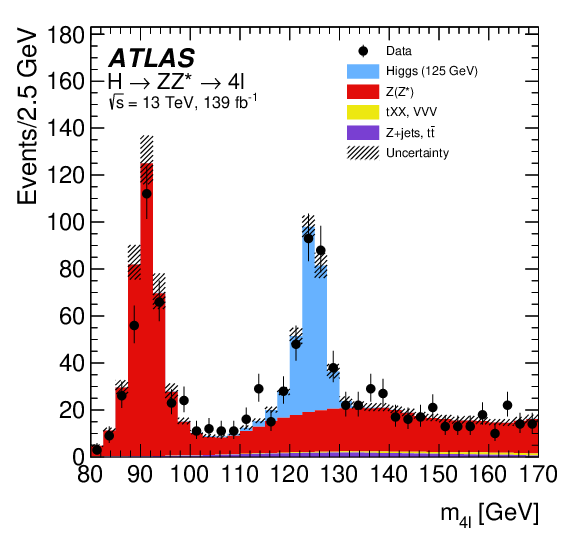
\includegraphics[width=0.42\textwidth]{Figures/mass4l_ATLAS.png}
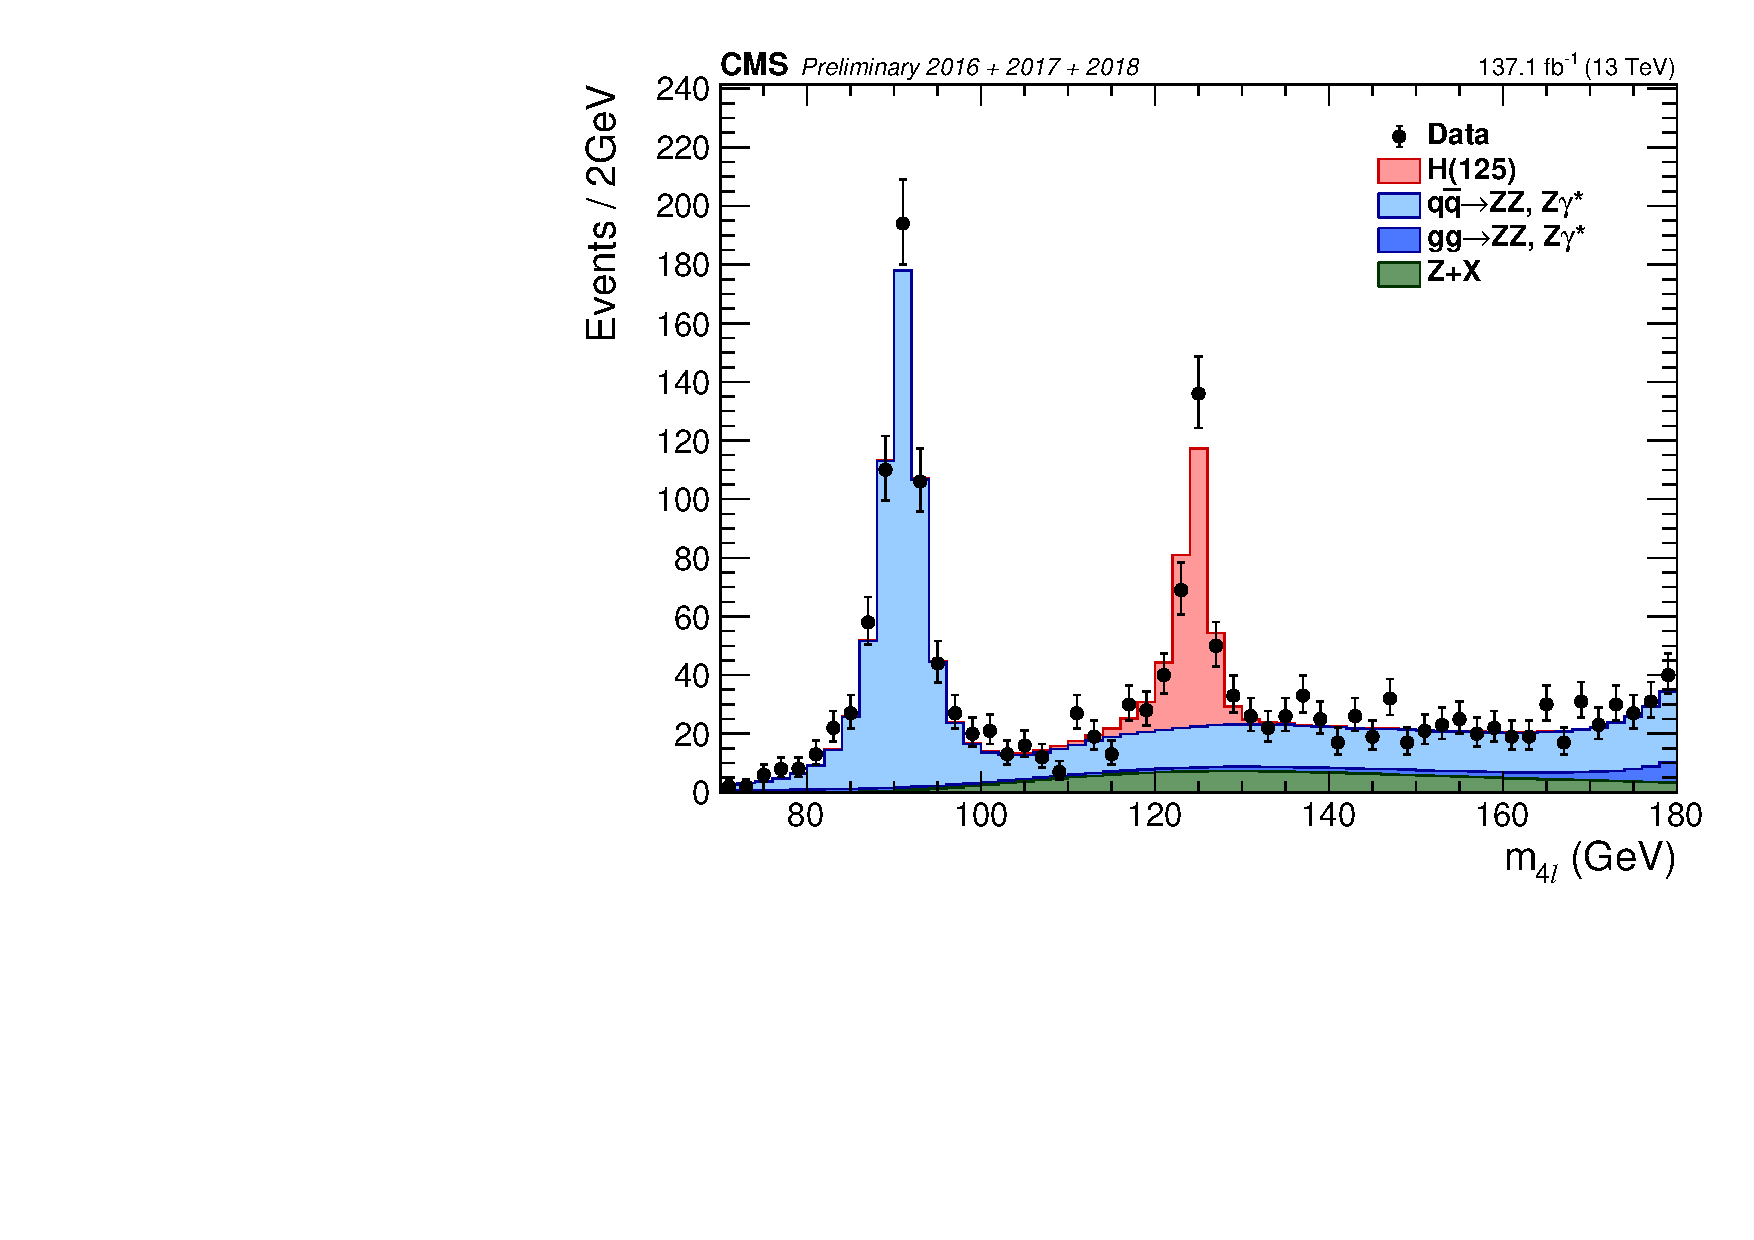
\includegraphics[width=0.53\textwidth]{Chapters/Chapter4/AnalysisStrategy/figures/Combination_lowMass.pdf}
	\caption{Left(Right): Reconstructed four-lepton invariant mass $\mfl$ at ATLAS (CMS) using an integrated luminosity of 139 $\ifb$ (137.1 $\ifb$).
\label{fig:distributions}}
\end{center}
\end{figure}

	The inclusive or integrated cross section as measured from ATLAS and CMS is given as $\sigma_{fid}=3.28\pm 0.32~ fb$ and $\sigma_{fid}=2.73^{+0.30}_{-0.29}=2.73^{+0.23}_{-0.22}({\rm stat.})^{+0.24}_{-0.19}({\rm syst.})~{\rm fb}$ respectively. 
	Inclusive cross section in different final state can be seen the Figure \ref{fig:inclusive_fid}.

	\begin{figure}[!htb]
\vspace*{0.3cm}
\begin{center}
%
\includegraphics[width=0.48\textwidth]{Figures/IrrBkg/Kfactor_qqZZ_mZZ.pdf}
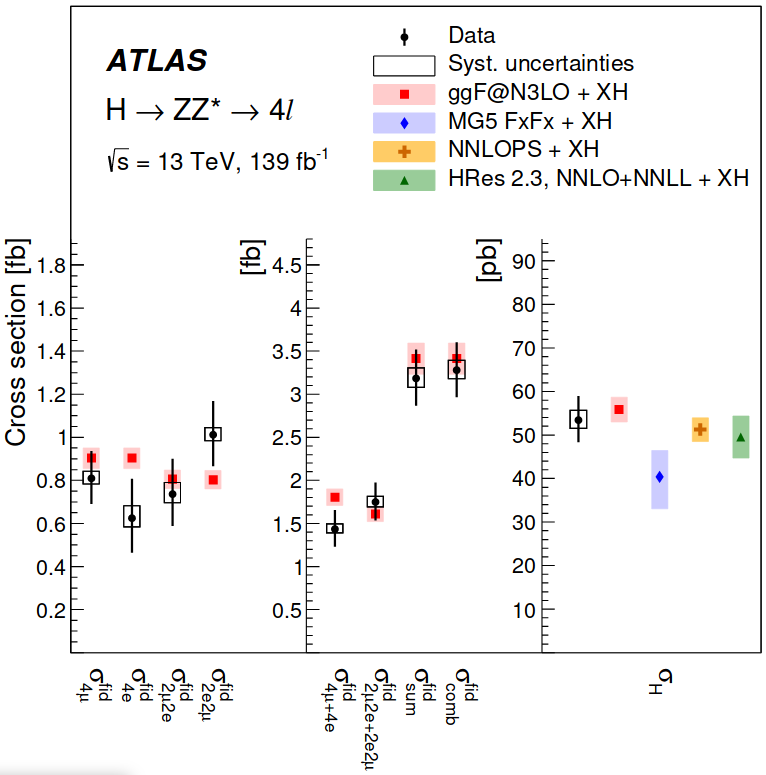
\includegraphics[width=0.43\textwidth]{Figures/ATLAS_fid.png}
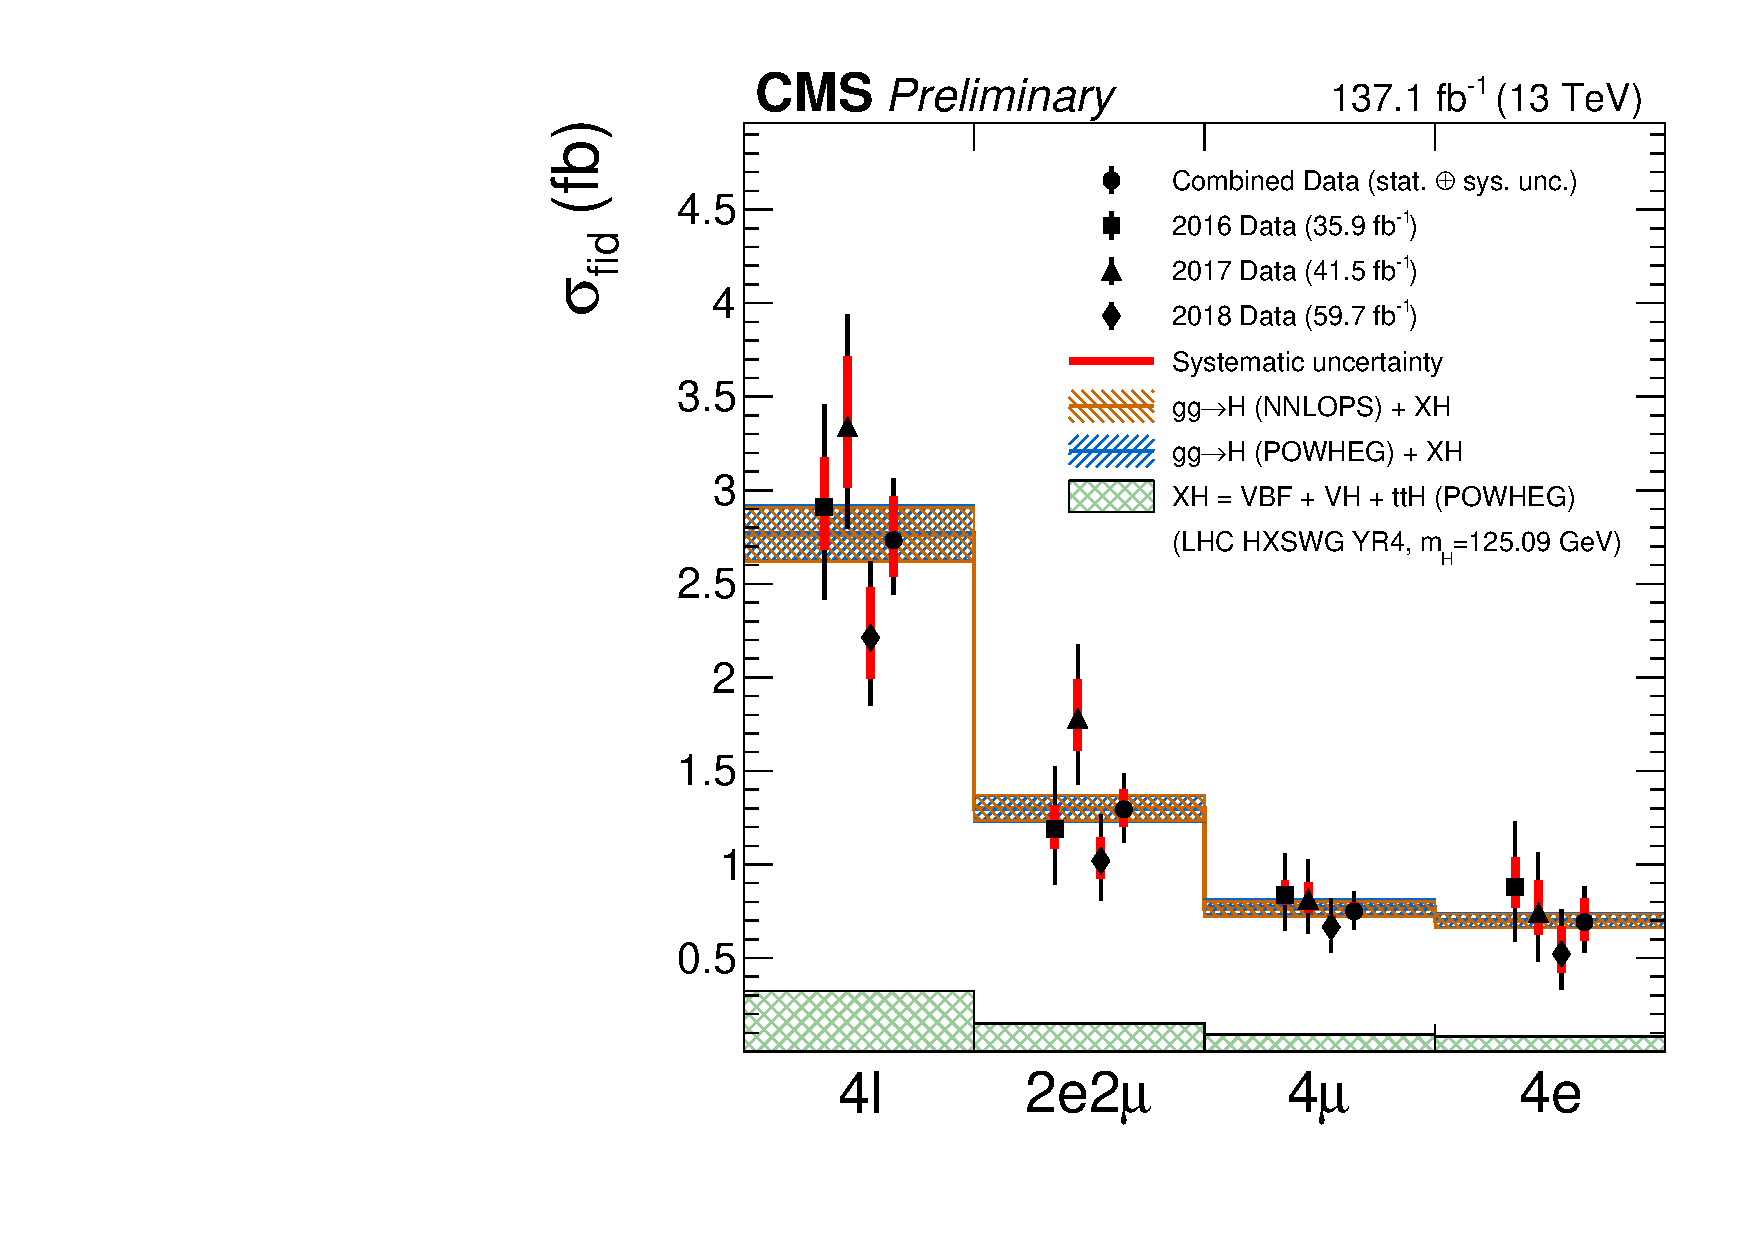
\includegraphics[width=0.47\textwidth]{Plots/mass4l_unfoldwith_SM_125_ThreeYears.pdf}
        \caption{Left(Right): Inclusive cross section in differential final states at ATLAS (CMS) using an integrated luminosity of 139 $\ifb$ (137.1 $\ifb$).
\label{fig:inclusive_fid}}
\end{center}
\end{figure}



	From CMS, current published results on differential cross section measurements in $H \rightarrow 4\ell$ decay channel, as described in the previous section, are based on production related observables which are four-leptons transverse momentum and rapidity, transverse momentum of leading jet, jet multiplicity. Therefore, the relevant bservables are compared from ATLAS measurements. In the following, differential measurements from ATLAS and CMS are shown side-by-side. (Figures \ref{fig:comp_pt4l}, \ref{fig:comp_rapidity4l}, \ref{fig:comp_njets} and \ref{fig:comp_pt_leading})

\begin{figure}[!htb]
\vspace*{0.3cm}
\begin{center}
%
\includegraphics[width=0.48\textwidth]{Figures/IrrBkg/Kfactor_qqZZ_mZZ.pdf}
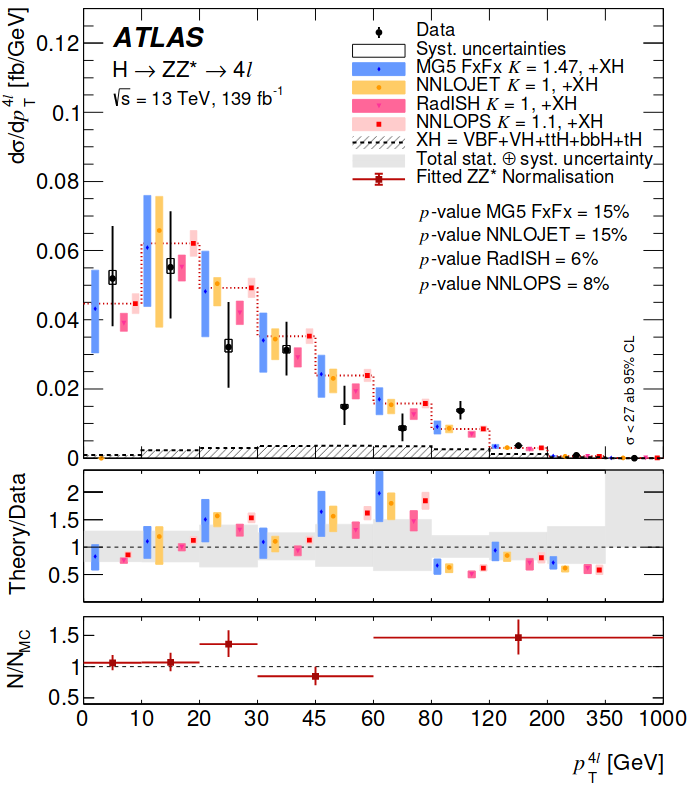
\includegraphics[width=0.43\textwidth]{Figures/ATLAS_pt4l.png}
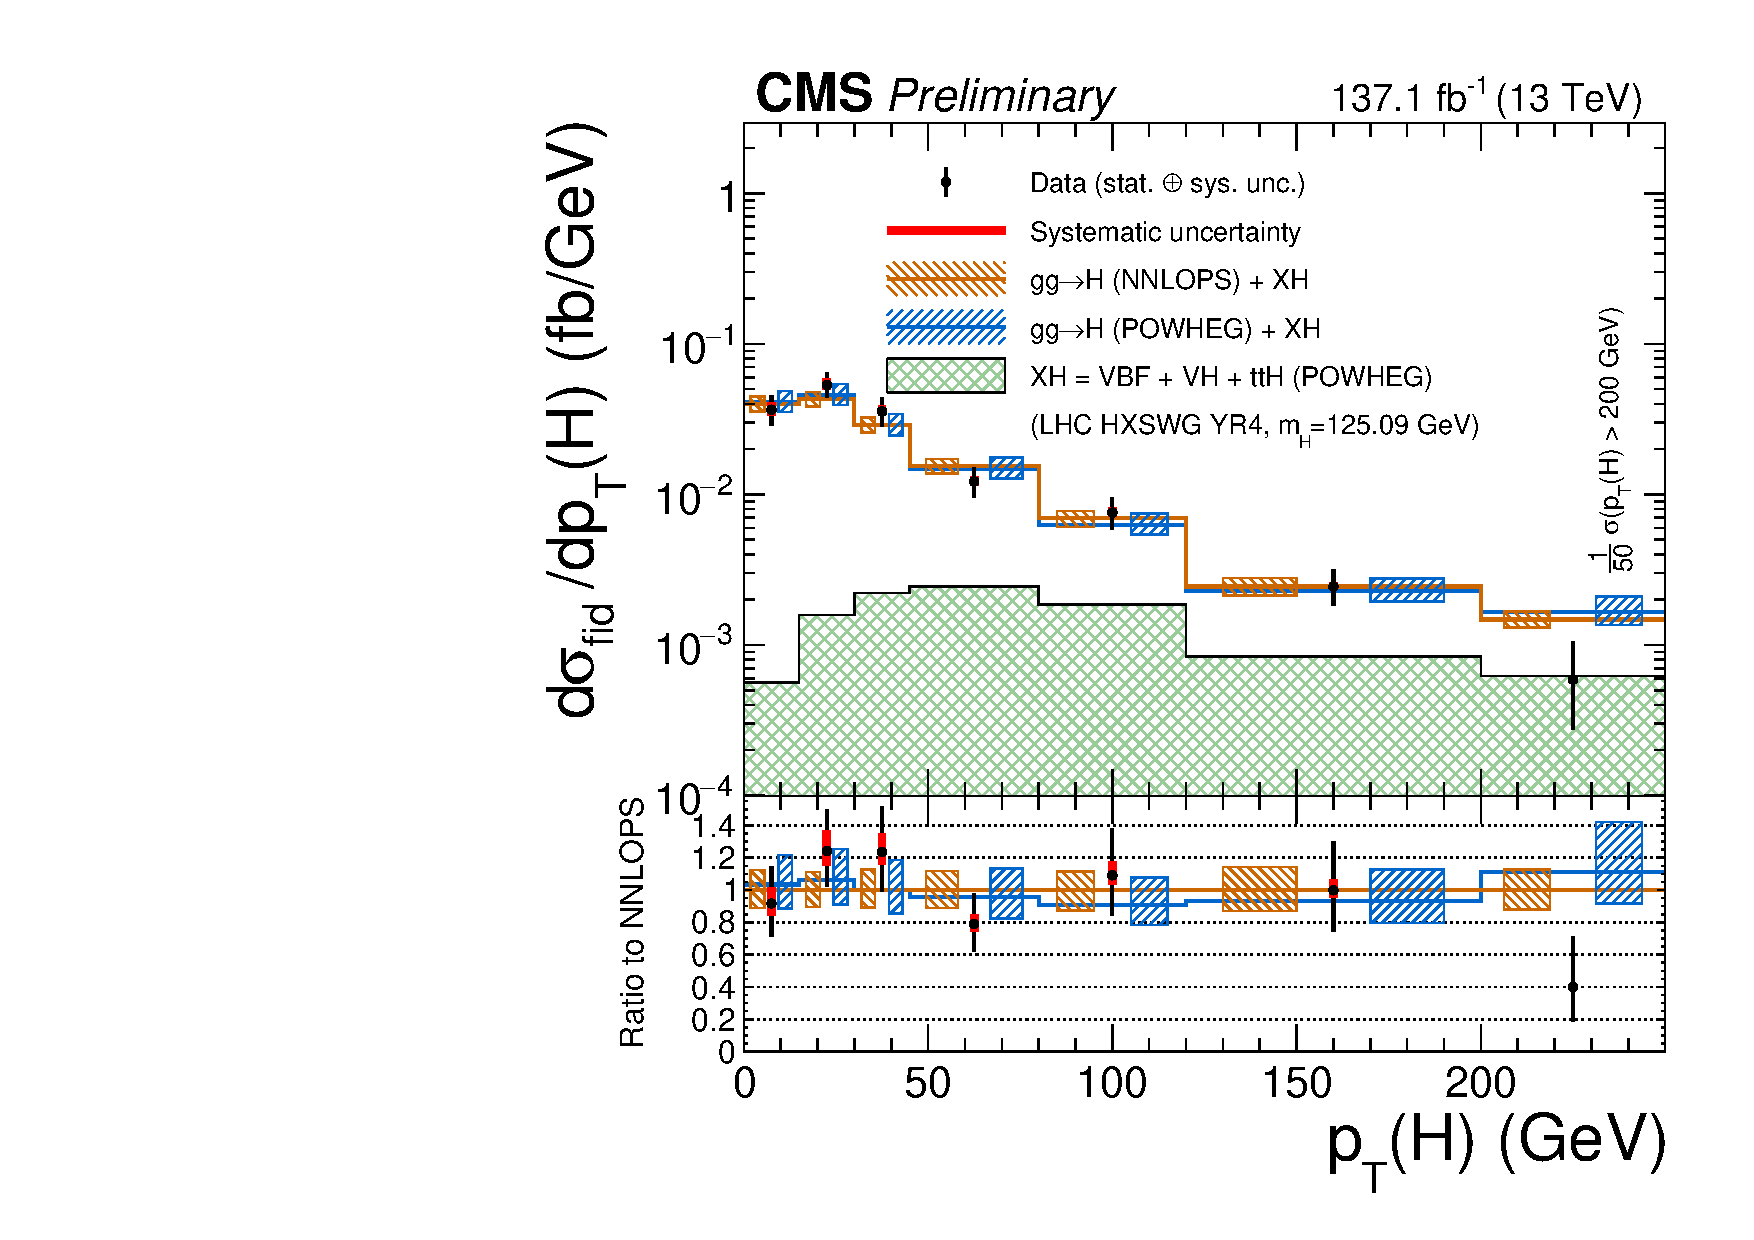
\includegraphics[width=0.47\textwidth]{Plots/pT4l_unfoldwith_SM_125_logscale.pdf}
	\caption{Left(Right): Higgs differential cross section as a function of transverse momentum of four lepton system with ATLAS (CMS) using an integrated luminosity of 139 $\ifb$ (137.1 $\ifb$). Results are shown with theory prediction in each experiment as described in \ref{theory_pred}.
\label{fig:comp_pt4l}}
\end{center}
\end{figure}


\begin{figure}[!htb]
\vspace*{0.3cm}
\begin{center}
%
\includegraphics[width=0.48\textwidth]{Figures/IrrBkg/Kfactor_qqZZ_mZZ.pdf}
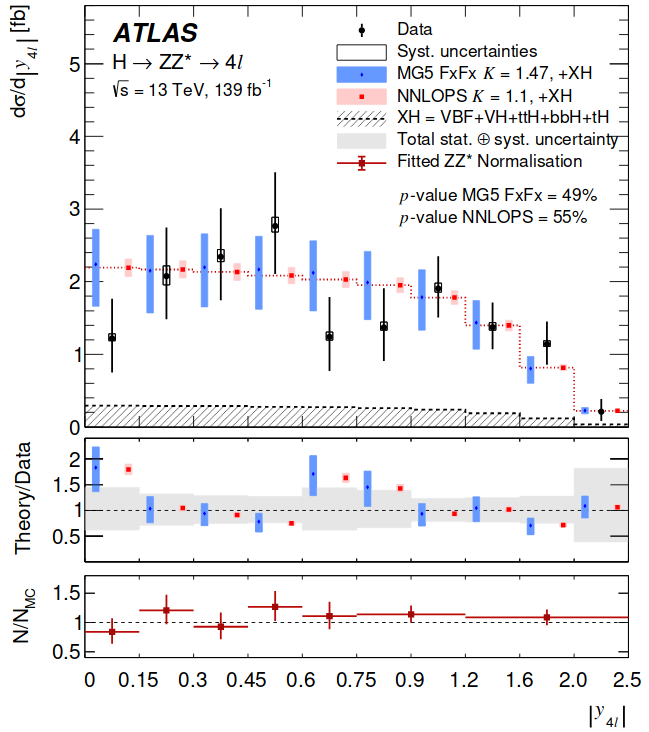
\includegraphics[width=0.43\textwidth]{Figures/ATLAS_rapidity4l.png}
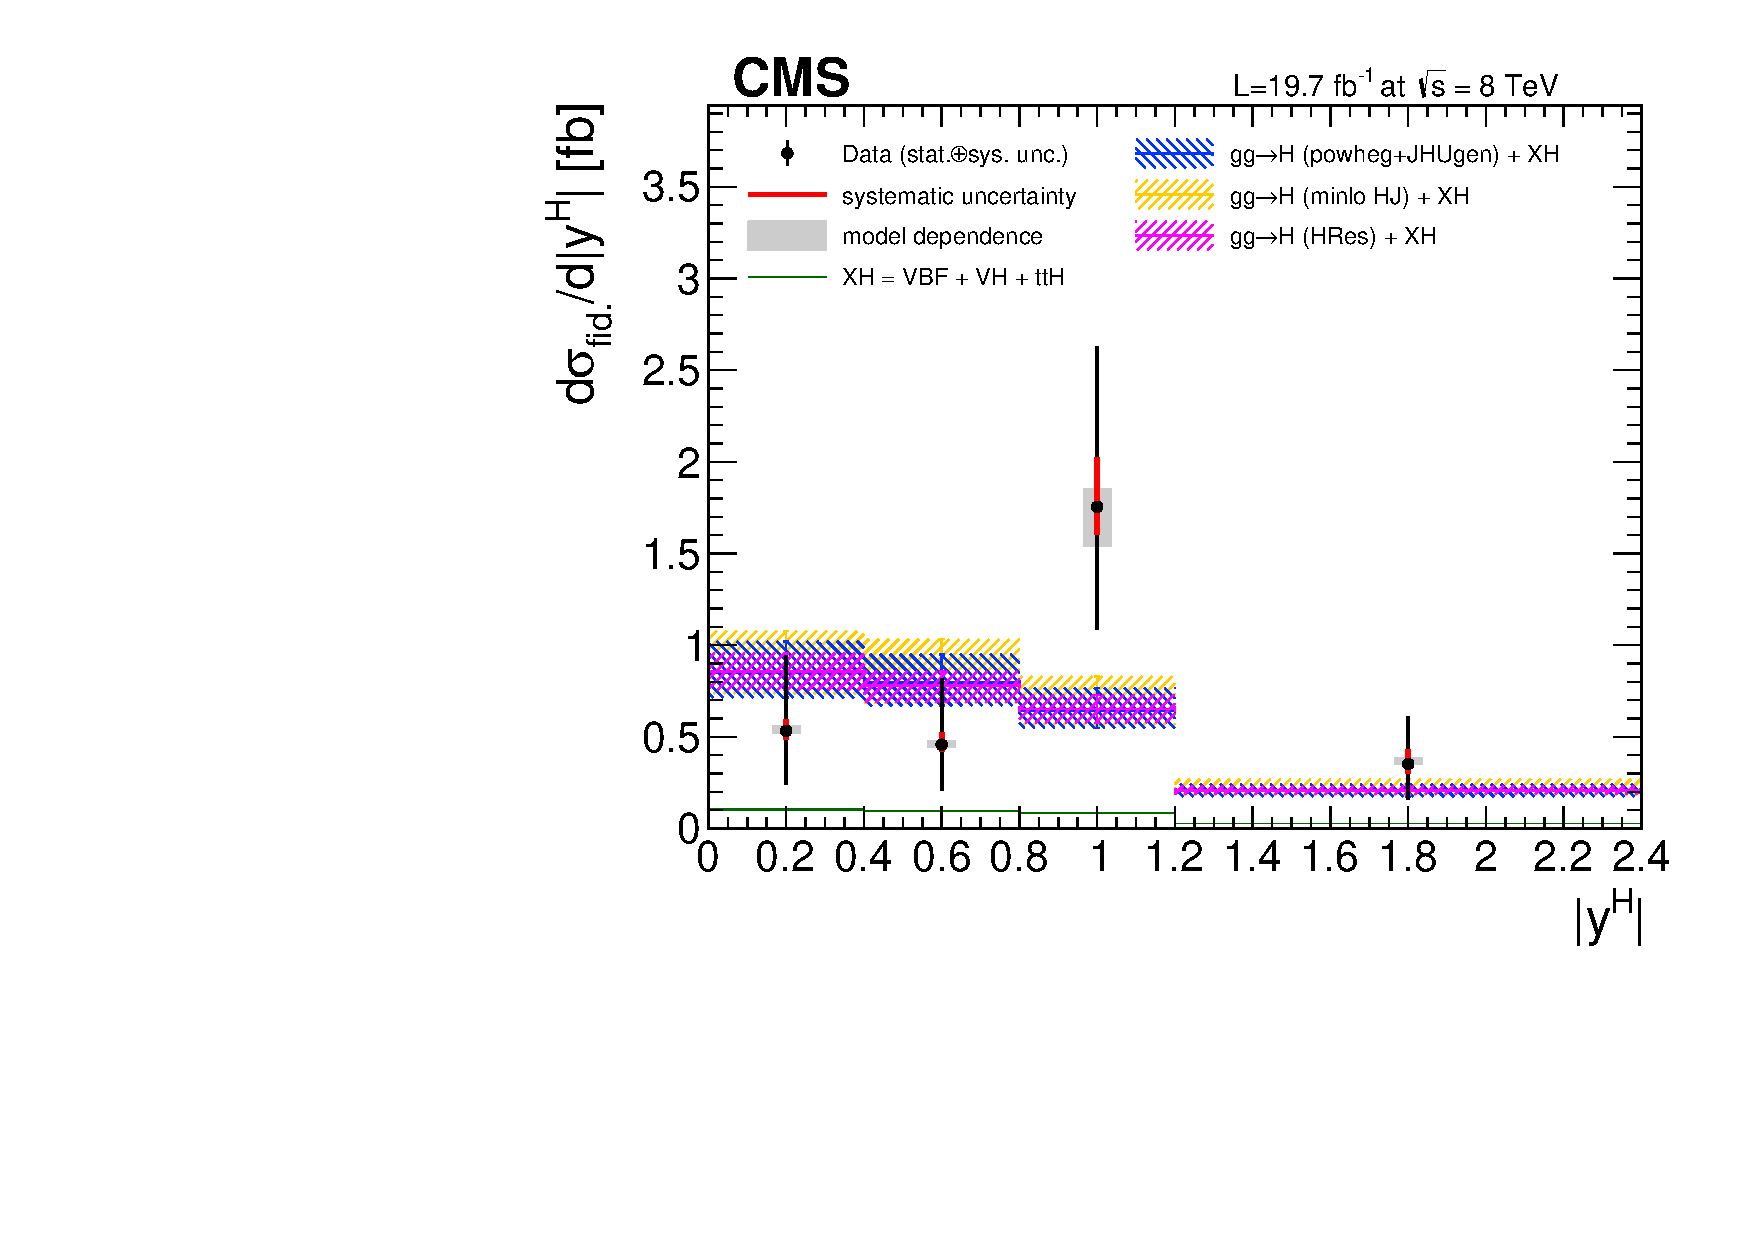
\includegraphics[width=0.47\textwidth]{Plots/rapidity4l_unfoldwith_SM_125.pdf}
        \caption{Left(Right): Higgs differential cross section as a function of rapidity of four lepton system  with ATLAS (CMS) using an integrated luminosity of 139 $\ifb$ (137.1 $\ifb$). Results are shown with theory prediction in each experiment as described in \ref{theory_pred}.
\label{fig:comp_rapidity4l}}
\end{center}
\end{figure}



\begin{figure}[!htb]
\vspace*{0.3cm}
\begin{center}
%
\includegraphics[width=0.48\textwidth]{Figures/IrrBkg/Kfactor_qqZZ_mZZ.pdf}
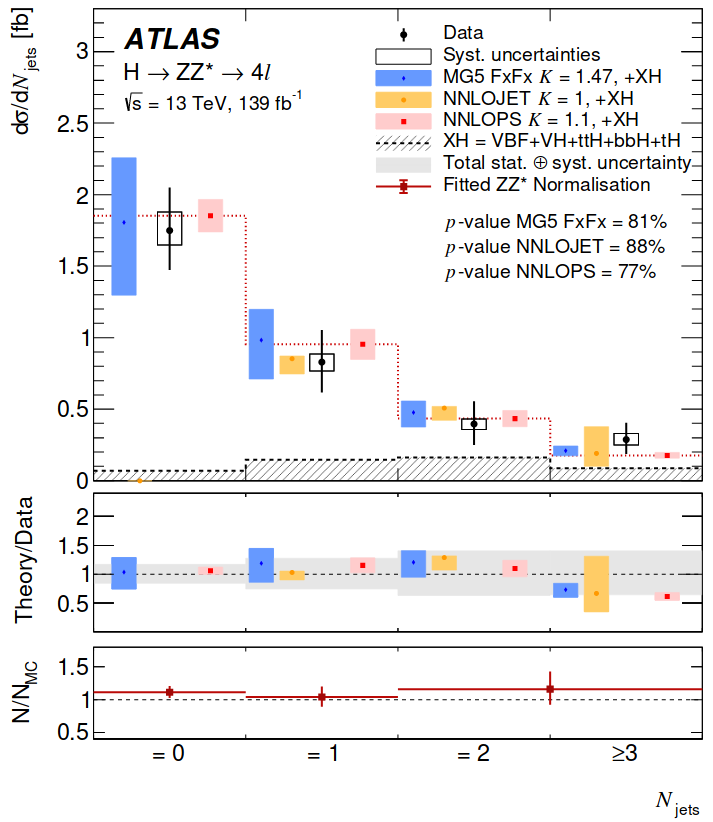
\includegraphics[width=0.43\textwidth]{Figures/ATLAS_njets.png}
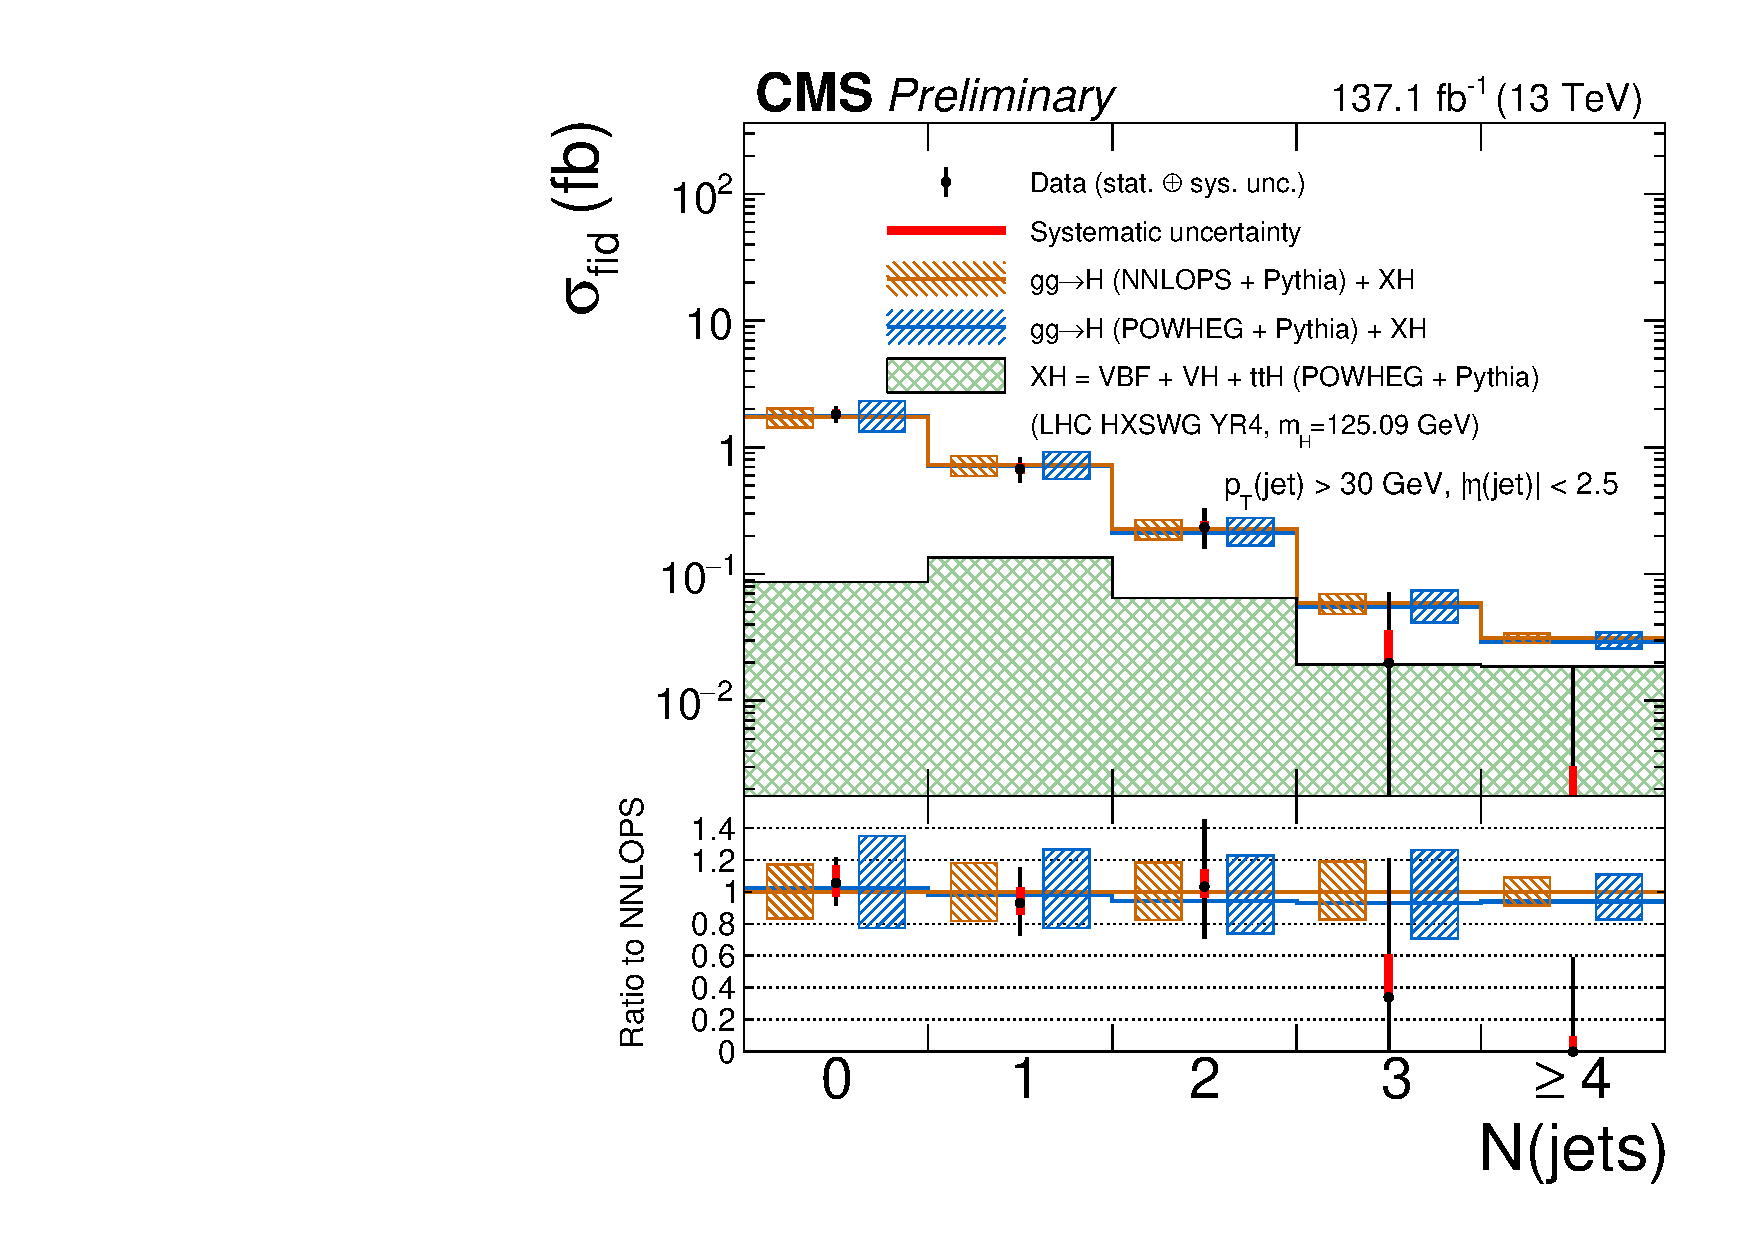
\includegraphics[width=0.47\textwidth]{Plots/njets_pt30_eta2p5_unfoldwith_SM_125_logscale.pdf}
        \caption{Left(Right): Higgs differential cross section as a function of jet multiplicity with  ATLAS (CMS) using an integrated luminosity of 139 $\ifb$ (137.1 $\ifb$). Results are shown with theory prediction in each experiment as described in \ref{theory_pred}.
\label{fig:comp_njets}}
\end{center}
\end{figure}


\begin{figure}[!htb]
\vspace*{0.3cm}
\begin{center}
%
\includegraphics[width=0.48\textwidth]{Figures/IrrBkg/Kfactor_qqZZ_mZZ.pdf}
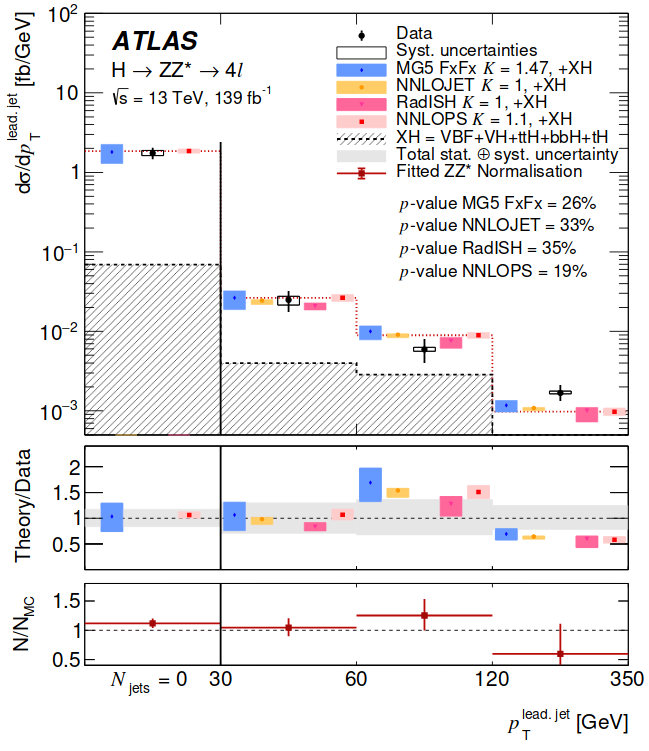
\includegraphics[width=0.43\textwidth]{Figures/ATLAS_pt_leading.png}
	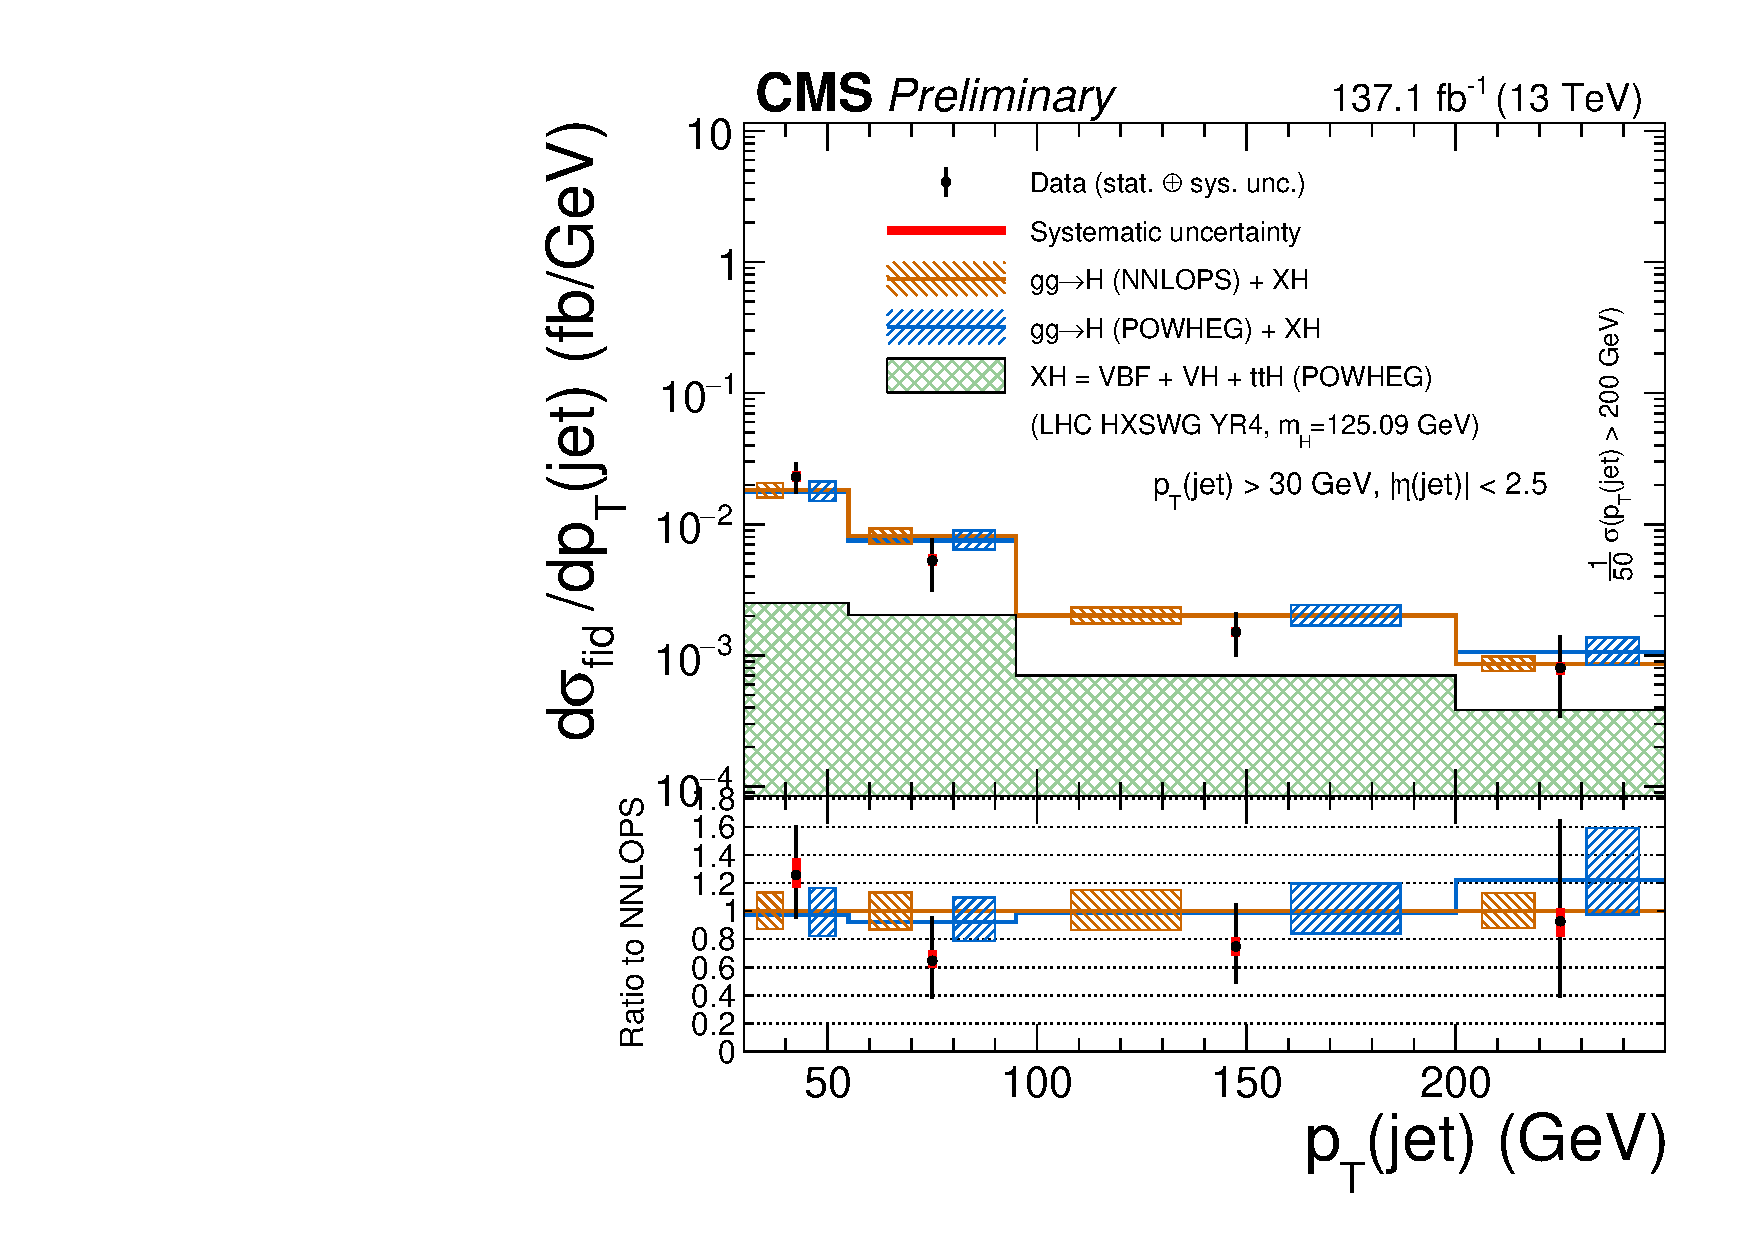
\includegraphics[width=0.47\textwidth]{Plots/pt_leadingjet_pt30_eta2p5_unfoldwith_SM_125_logscale.pdf}
        \caption{Left(Right): Higgs differential cross section as a function of transverse momentum of the leading jet with  ATLAS (CMS) using an integrated luminosity of 139 $\ifb$ (137.1 $\ifb$). Results are shown with theory prediction in each experiment as described in \ref{theory_pred}.
\label{fig:comp_pt_leading}}
\end{center}
\end{figure}
	
	%	
%(Y(H)- Y(leading jet) chosen by CMS ). Figure \ref{fig:ATLAS_differential-bins-2} shows the differential cross section results as function of differential 
%observables. The integrated fiducial production cross section was measured to be 
%$\sigma_{{\rm fid.}}^{{\rem tot.}}=2.11^{+0.53}_{-0.47}$(stat.)$\pm 0.08$(syst.) fb while the theoretical prediction at estimated for Higgs boson mass of 125.4~GeV
%is $1.30\pm0.13$~fb. Both ATLAS and CMS measurements are found to be compatible with theoretical estimations and no significant deviation has been observed. 
%The p-value are  obtained for differential observable N(jets) ( largest deviation from the SM based predictions was observed in case of the CMS)   
%$p = 0.13 (0.37)$ for the CMS (ATLAS).
%% However, 
%% compatibility p-value was found to be less  
%\begin{figure}[!h!tb]
%  \begin{center}
%    \subfigure[$\pt(\mathrm{H})$]{
%      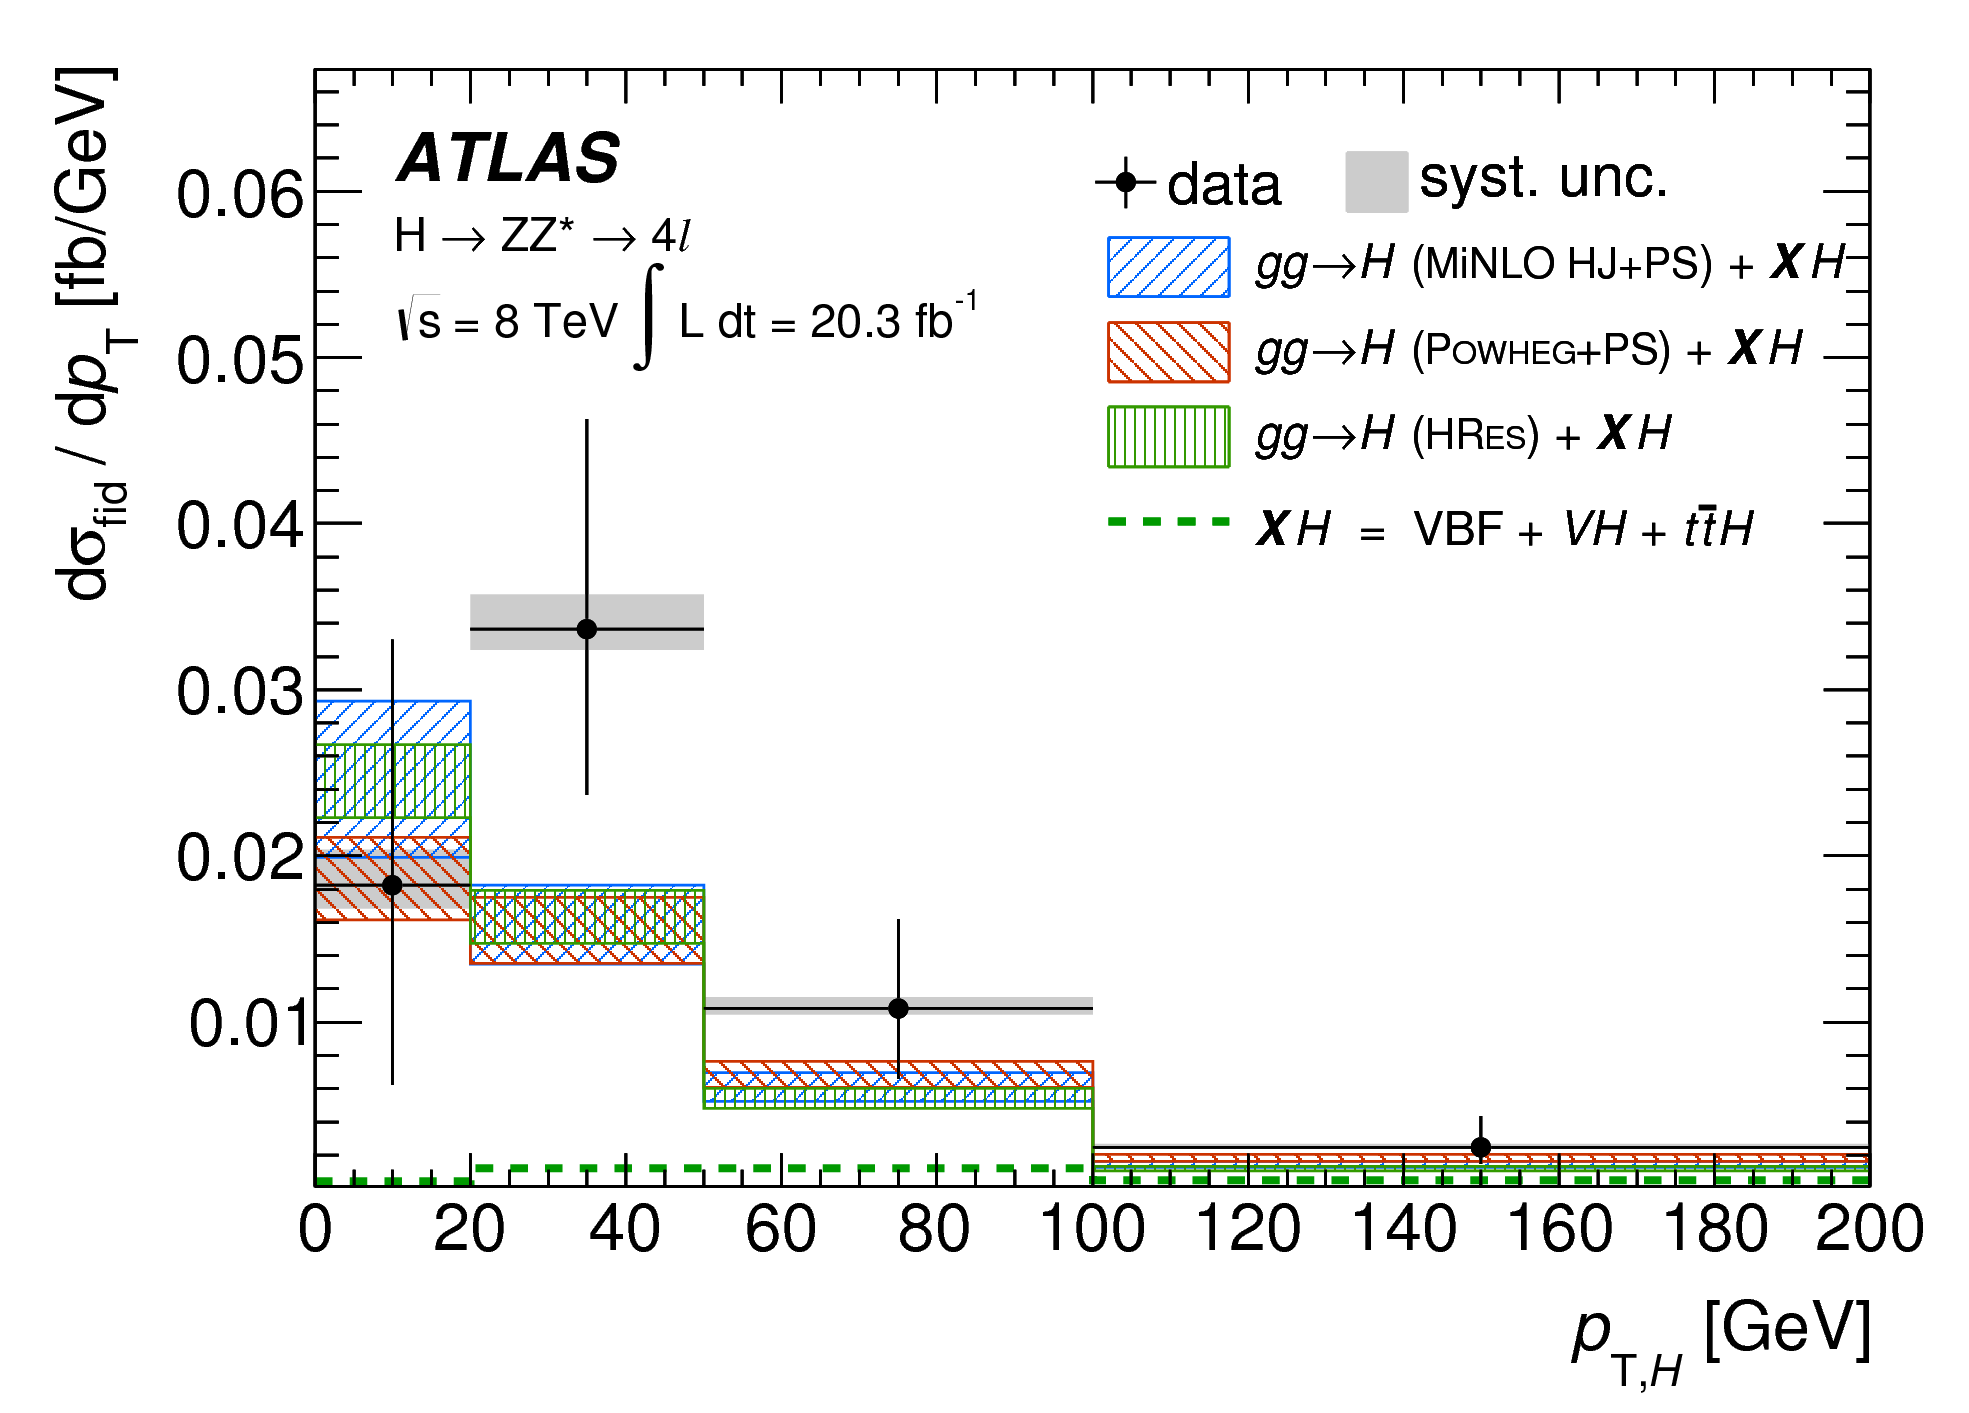
\includegraphics[width=0.45\textwidth,angle=0]{ATLAS_results/fig_02a.png}
%      \label{fig:ATLAS_differential-bins-2:a}
%    }
%    \subfigure[$|y(\mathrm{H})|$]{
%      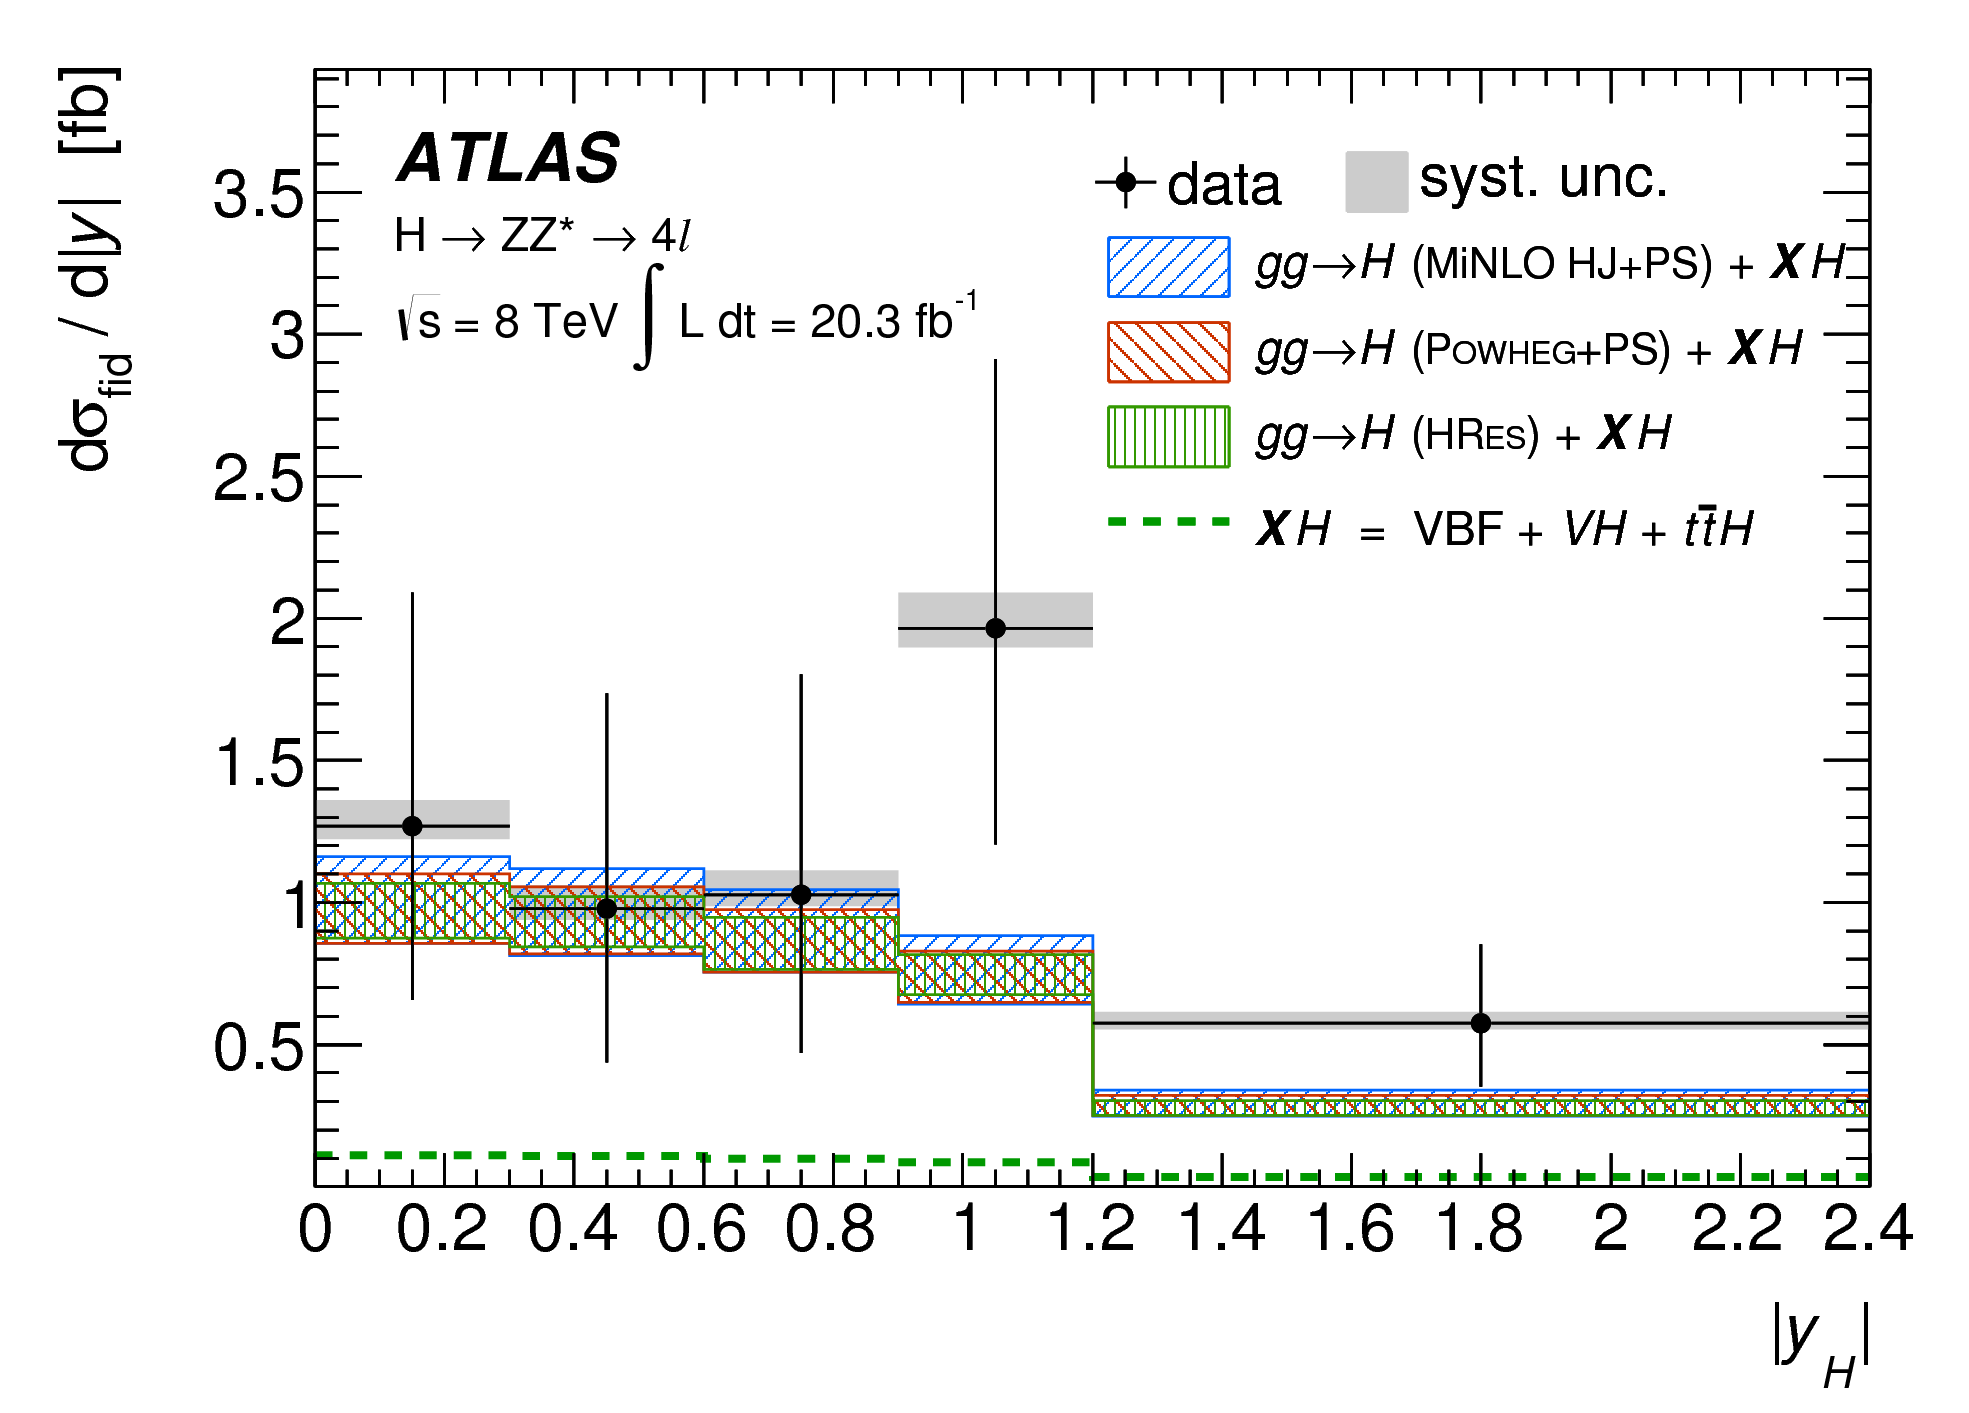
\includegraphics[width=0.45\textwidth,angle=0]{ATLAS_results/fig_02b.png}
%      \label{fig:ATLAS_differential-bins-2:b}
%    }
%    \subfigure[$\mathrm{m}(\mathrm{Z}_{2})$]{
%      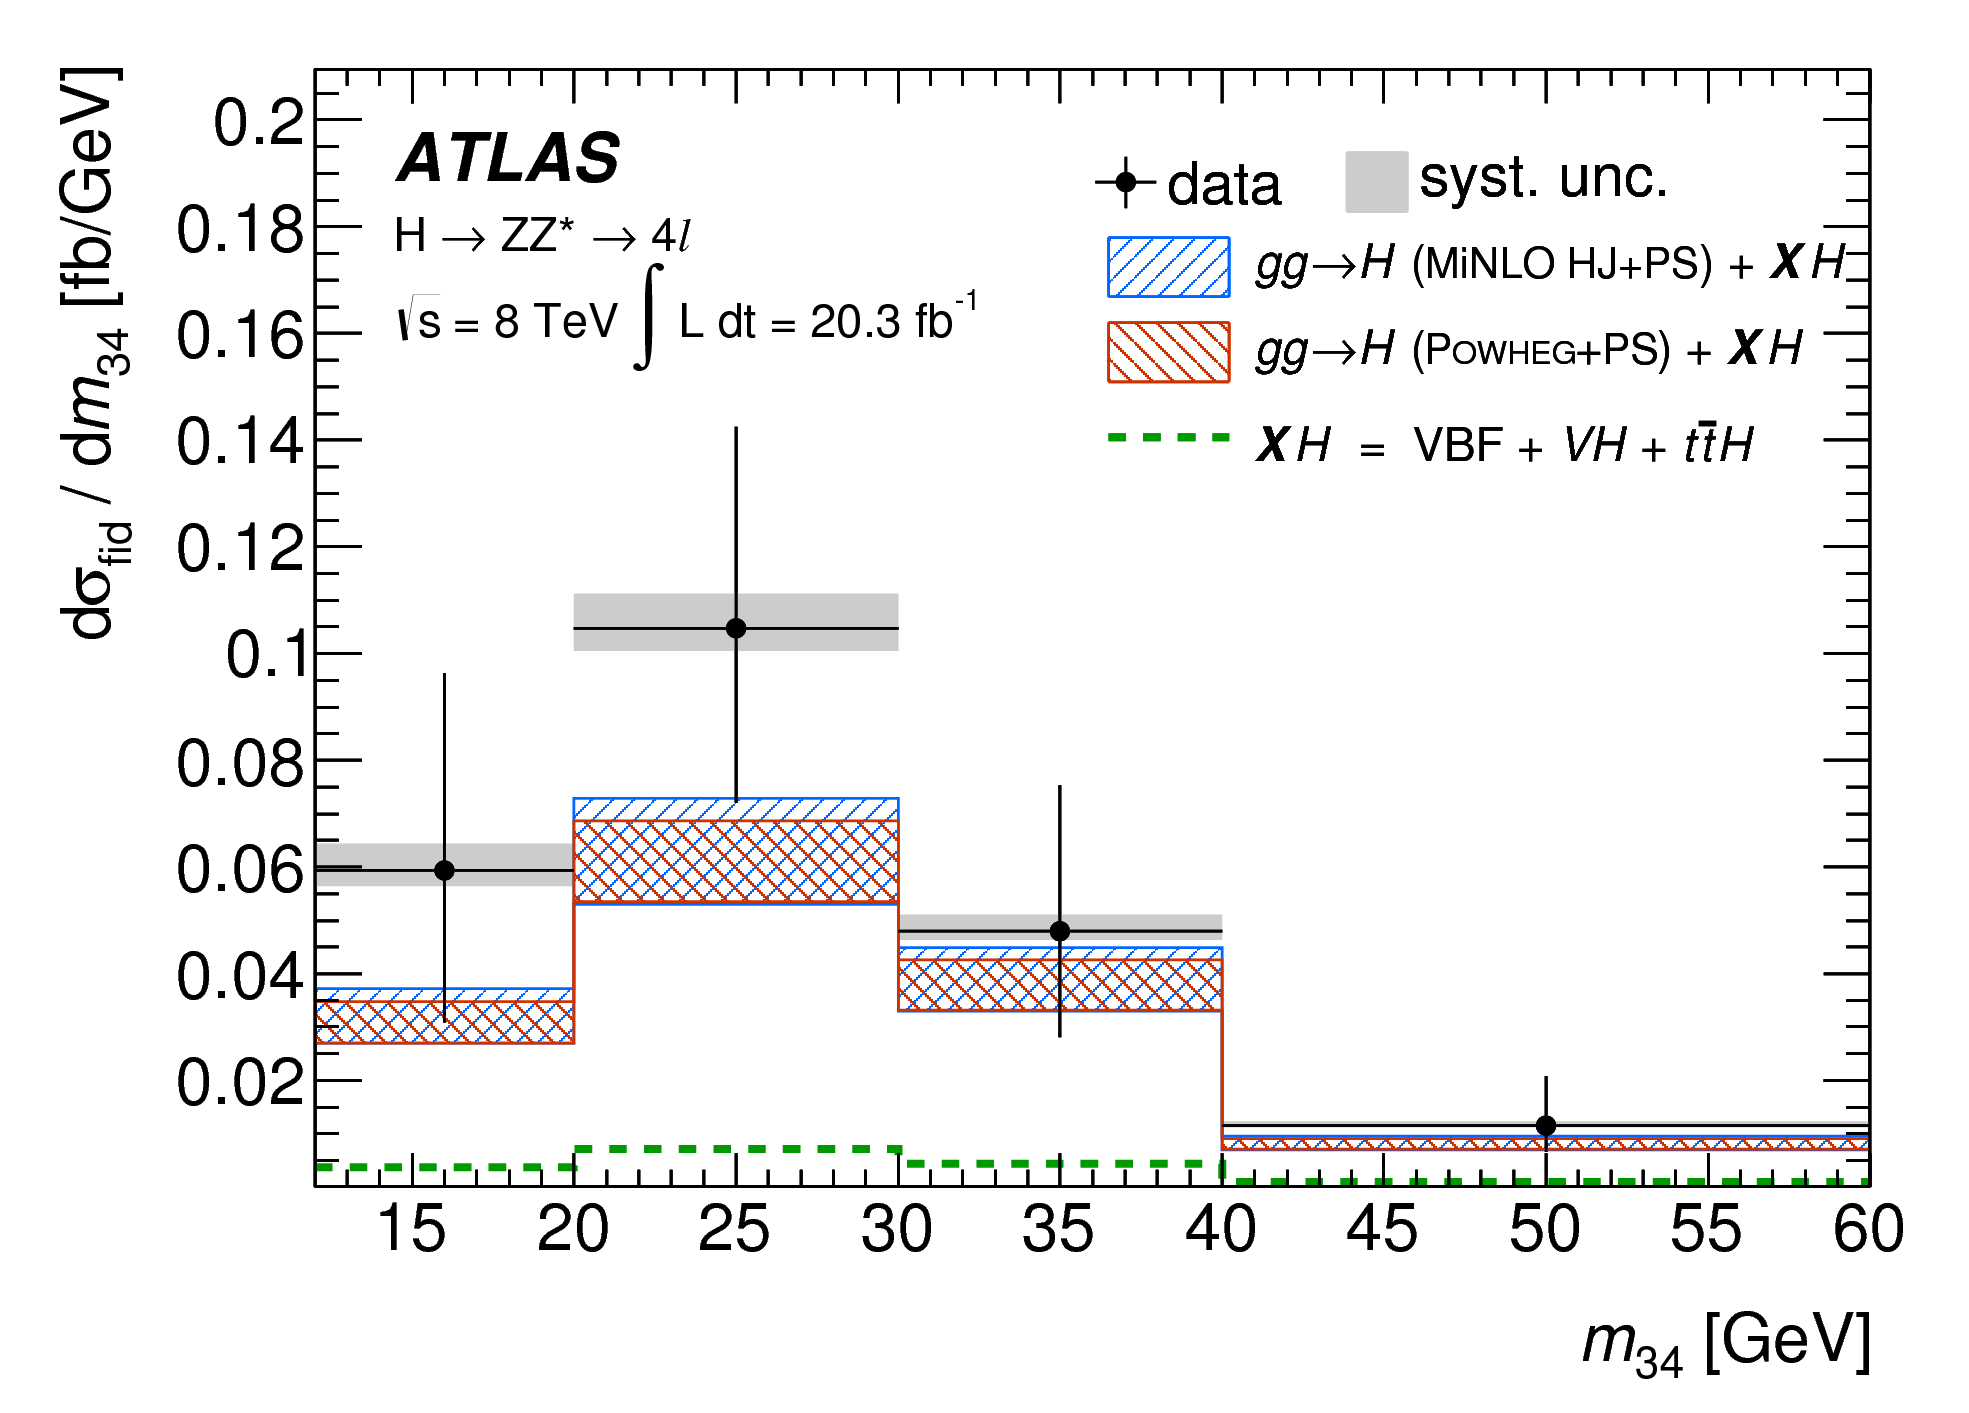
\includegraphics[width=0.45\textwidth,angle=0]{ATLAS_results/fig_02c.png}
%      \label{fig:ATLAS_differential-bins-2:c}
%    } 
%    \subfigure[$|\cos \theta^{*}|$]{
%      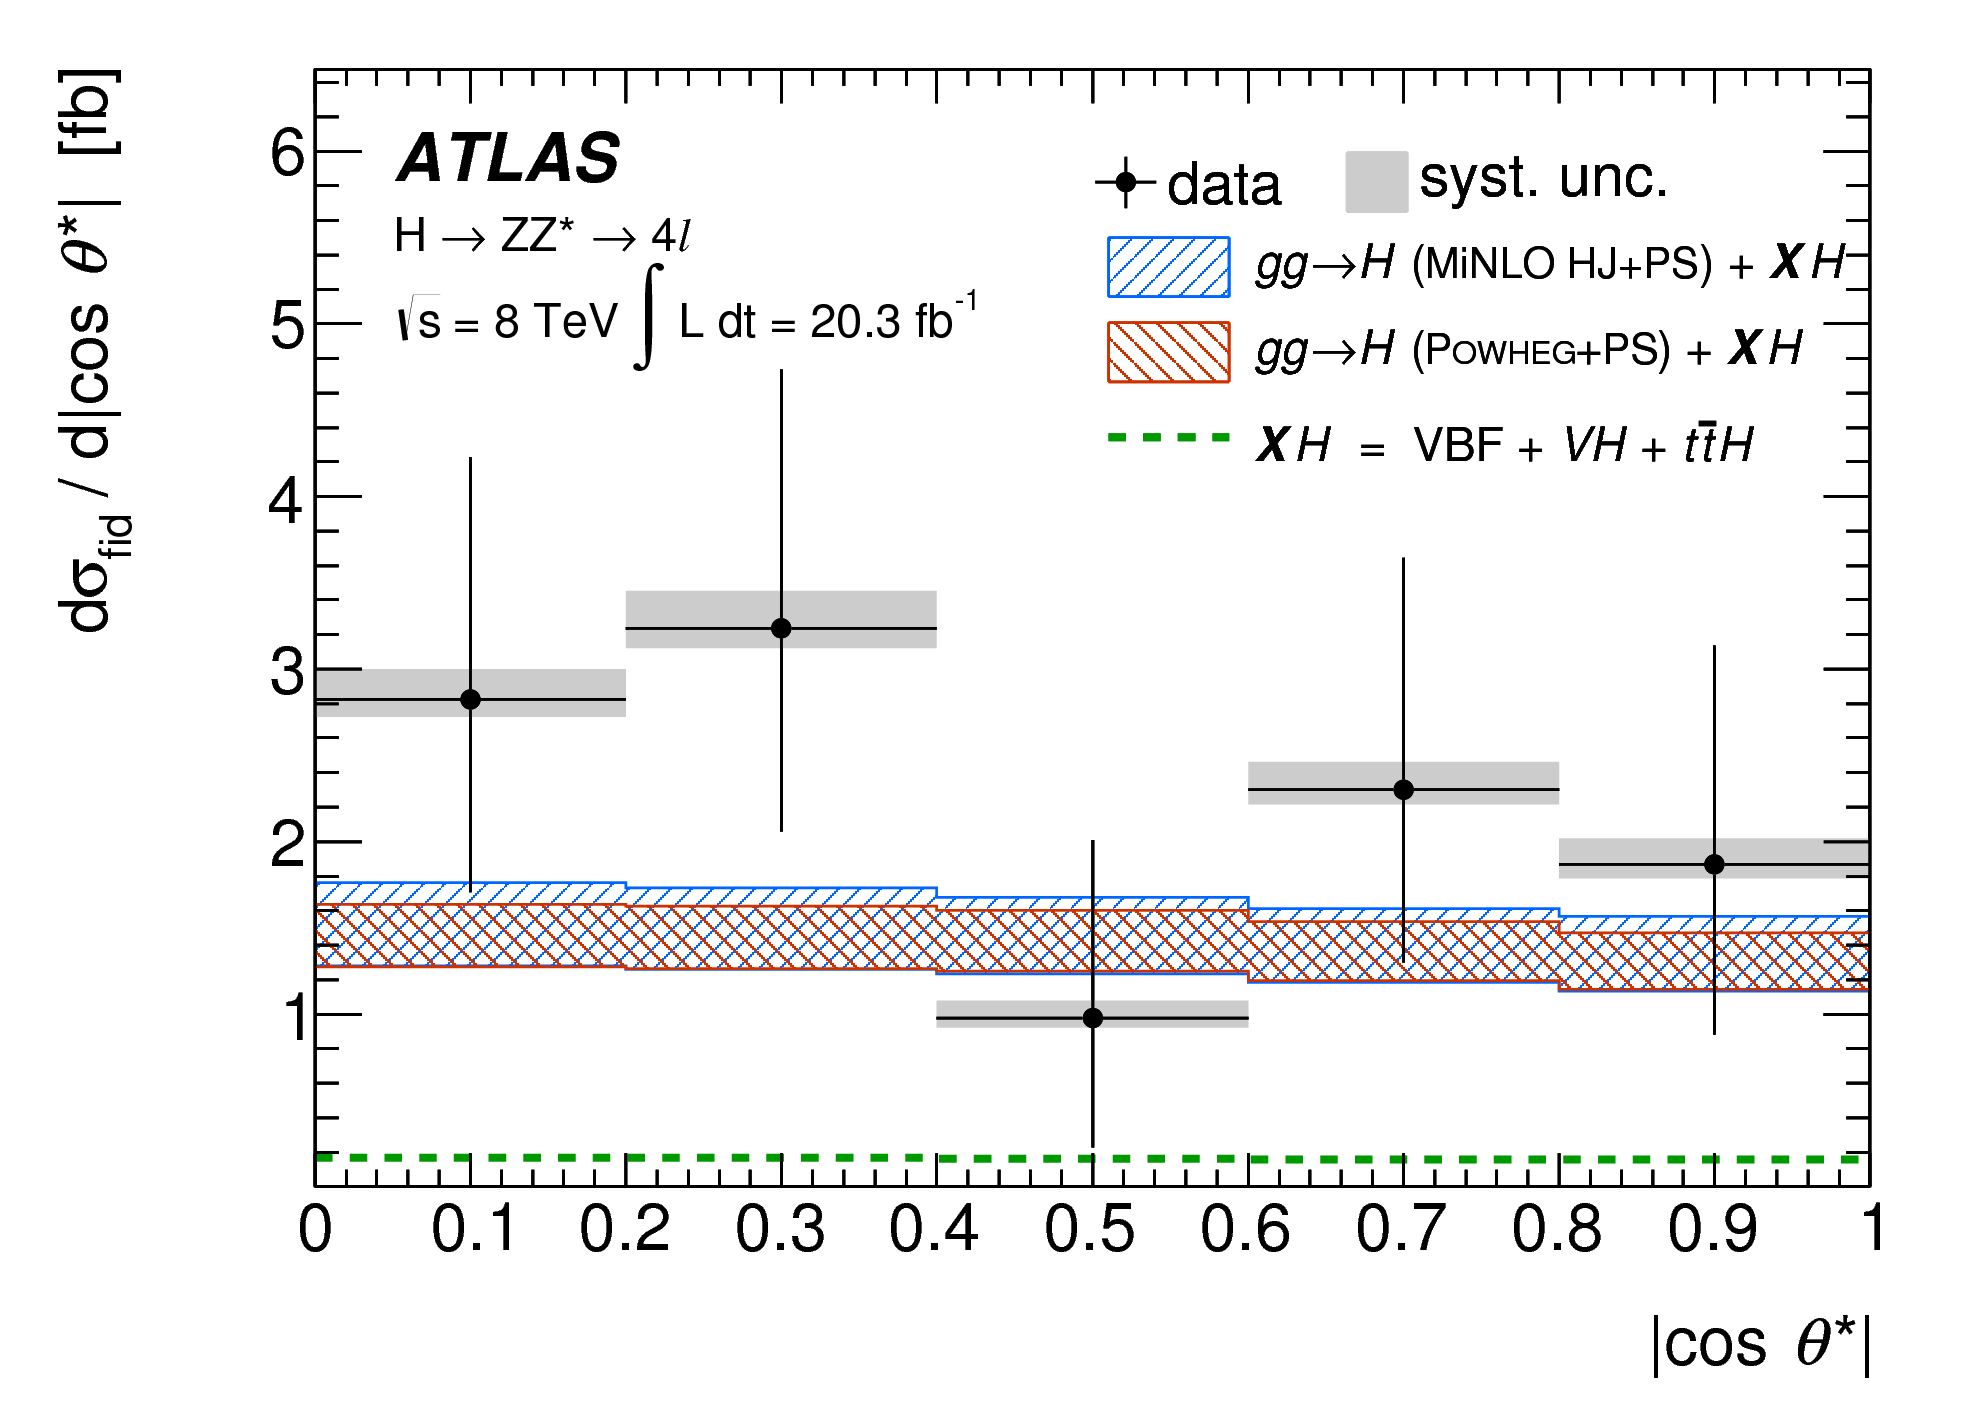
\includegraphics[width=0.45\textwidth,angle=0]{ATLAS_results/fig_02d.png}
%      \label{fig:ATLAS_differential-bins-2:d}
%    }
%    \subfigure[N(jets)]{
%      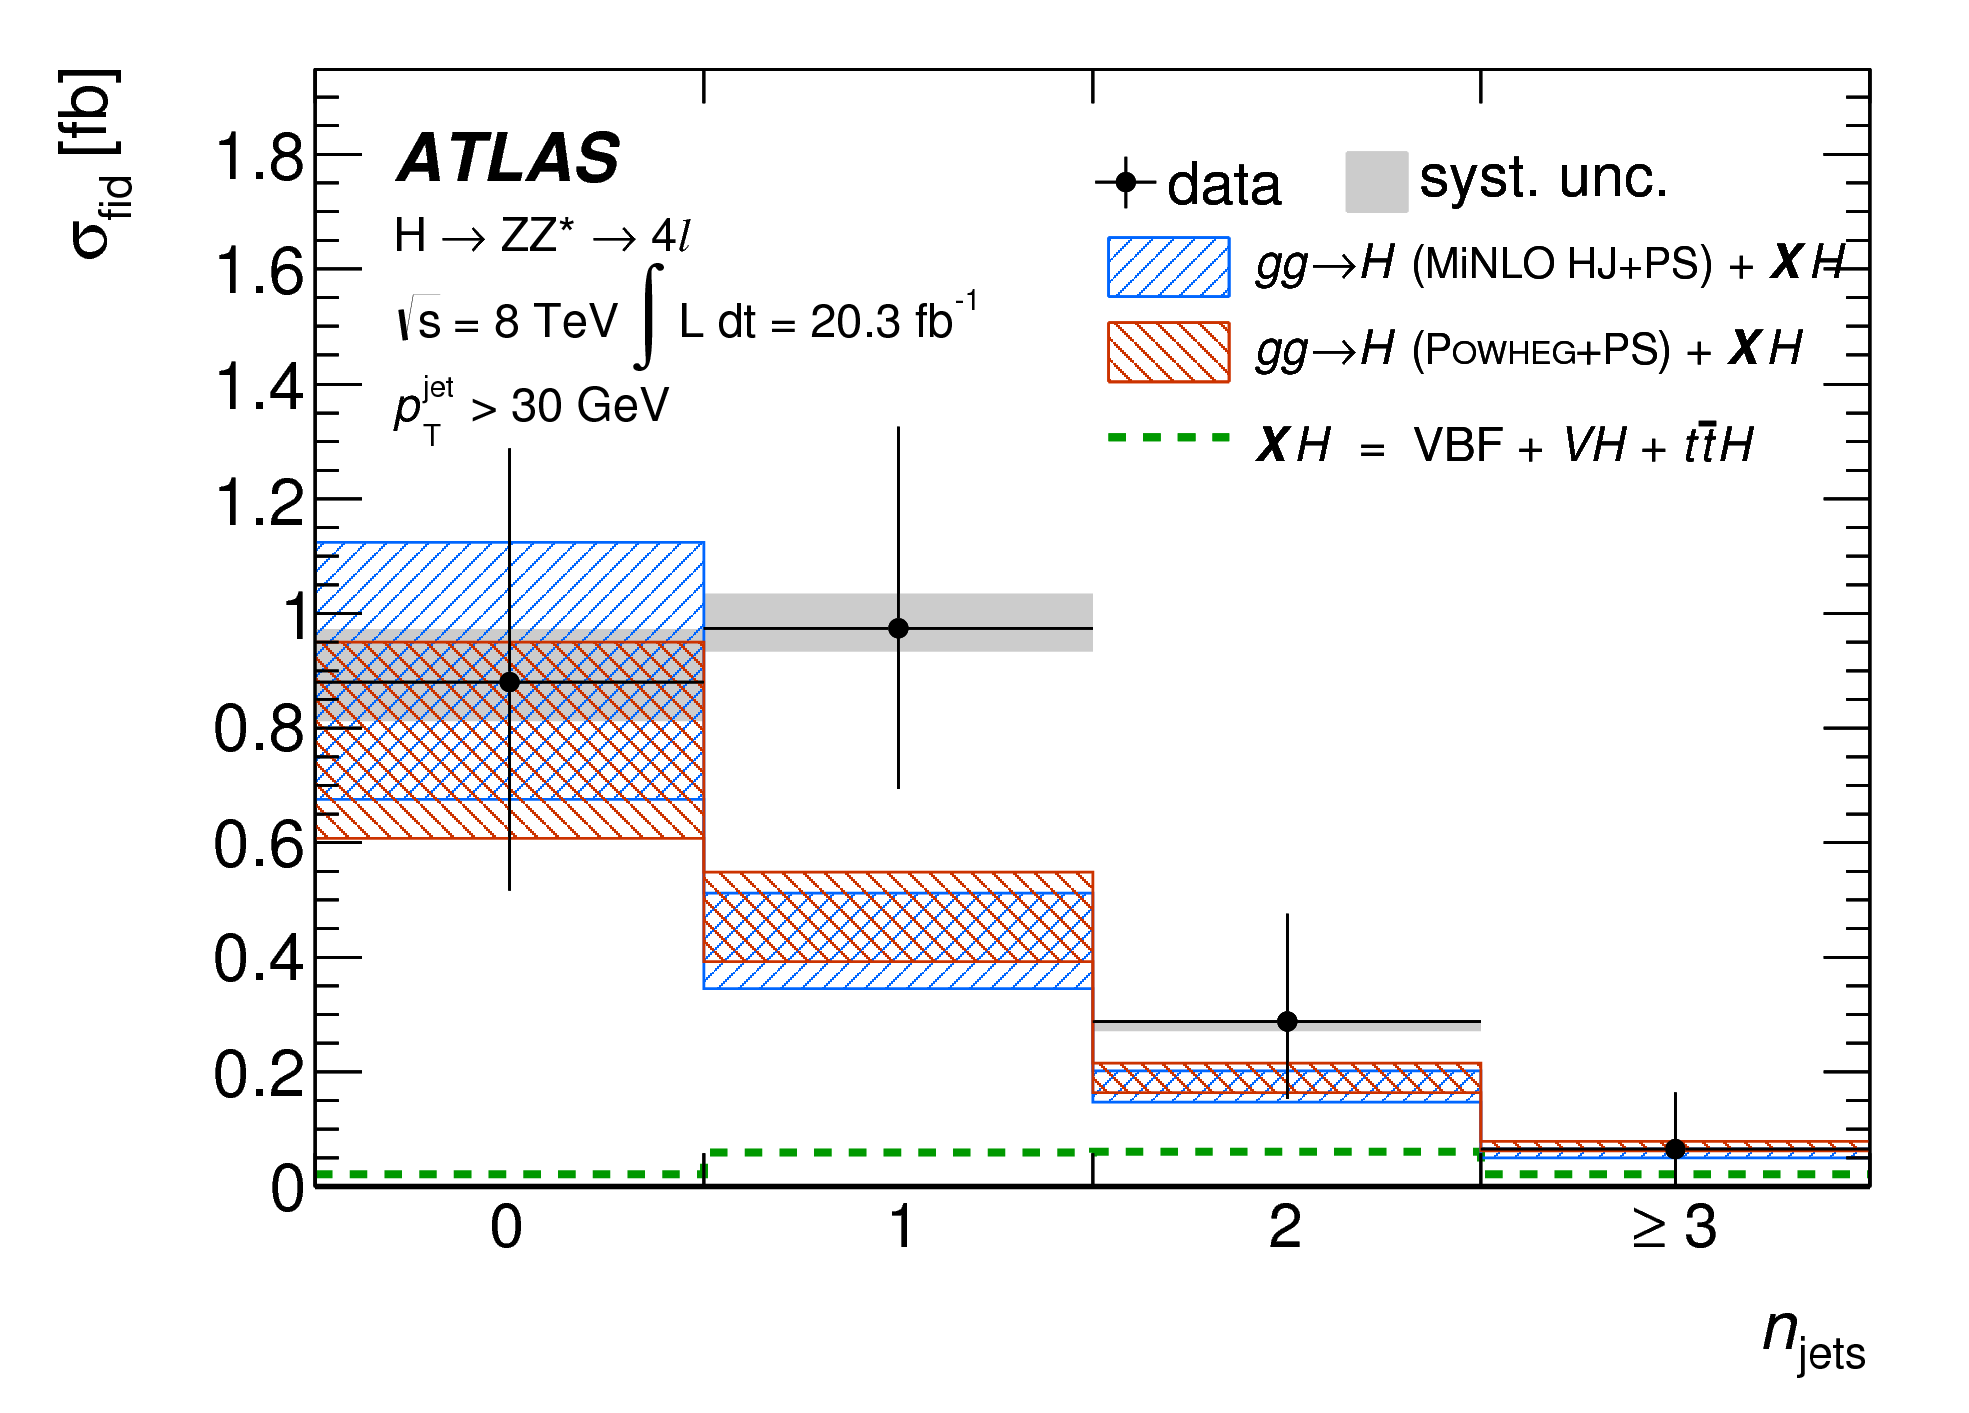
\includegraphics[width=0.45\textwidth,angle=0]{ATLAS_results/fig_02e.png}
%      \label{fig:ATLAS_differential-bins-2:e}                             
%    }
%    \subfigure[$\pt(\mathrm{jet})$]{
%      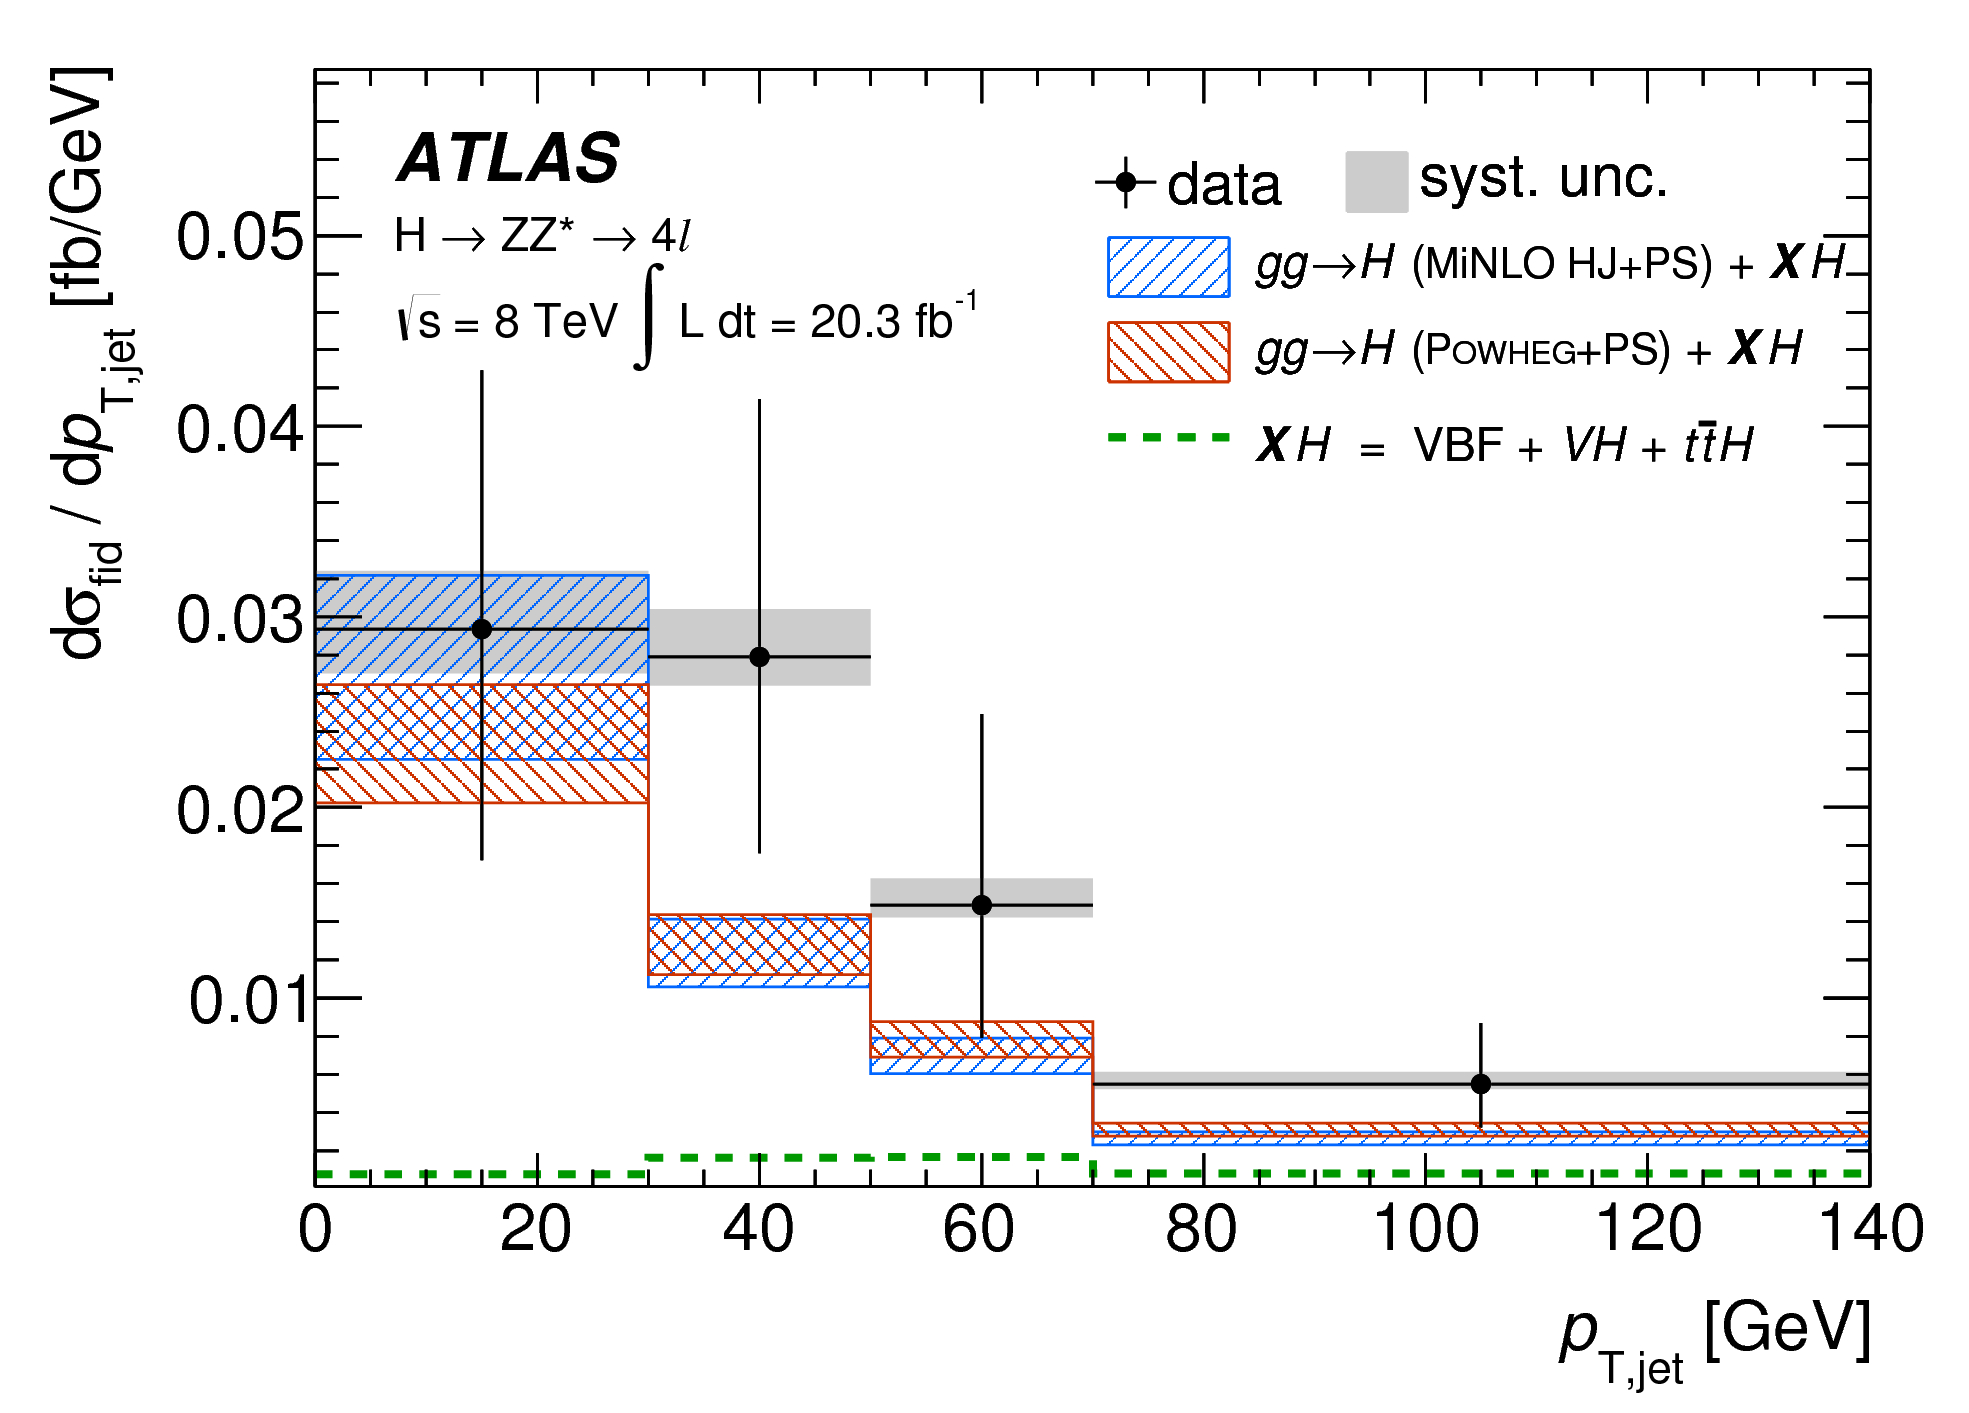
\includegraphics[width=0.45\textwidth,angle=0]{ATLAS_results/fig_02f.png}
%      \label{fig:ATLAS_differential-bins:f}
%    }
%    \caption{Observed data along with the SM signal (m(H)=$125.0 \GeV$) and background expectations for different observables
%    and for all final states combined, in range $105 < m_{4\ell} < 140 \GeV$ used for the $\Hllll$ measurements. The extraction of the 
%    signal is performed by exploiting the differences in the expected $m_{4\ell}$ spectra of the signal and background contributions in
%    each bin of an observable.
%    }
%  \label{fig:ATLAS_differential-bins-2}
% \end{center}
%\end{figure}
